%%%%%%%%%%%%%%%%%%%%%%%%%%%%%%%%%%%%%%%%%
% Masters/Doctoral Thesis 
% LaTeX Template
% Version 2.5 (27/8/17)
%
% This template was downloaded from:
% http://www.LaTeXTemplates.com
%
% Version 2.x major modifications by:
% Vel (vel@latextemplates.com)
%
% This template is based on a template by:
% Steve Gunn (http://users.ecs.soton.ac.uk/srg/softwaretools/document/templates/)
% Sunil Patel (http://www.sunilpatel.co.uk/thesis-template/)
%
% Template license:
% CC BY-NC-SA 3.0 (http://creativecommons.org/licenses/by-nc-sa/3.0/)
%
%%%%%%%%%%%%%%%%%%%%%%%%%%%%%%%%%%%%%%%%%

%----------------------------------------------------------------------------------------
%	PACKAGES AND OTHER DOCUMENT CONFIGURATIONS
%----------------------------------------------------------------------------------------

\documentclass[
11pt, % The default document font size, options: 10pt, 11pt, 12pt
%oneside, % Two side (alternating margins) for binding by default, uncomment to switch to one side
english, % ngerman for German
doublespacing, %singlespacing, % Single line spacing, alternatives: onehalfspacing or doublespacing
%draft, % Uncomment to enable draft mode (no pictures, no links, overfull hboxes indicated)
%nolistspacing, % If the document is onehalfspacing or doublespacing, uncomment this to set spacing in lists to single
%liststotoc, % Uncomment to add the list of figures/tables/etc to the table of contents
%toctotoc, % Uncomment to add the main table of contents to the table of contents
%parskip, % Uncomment to add space between paragraphs
%nohyperref, % Uncomment to not load the hyperref package
headsepline, % Uncomment to get a line under the header
%chapterinoneline, % Uncomment to place the chapter title next to the number on one line
%consistentlayout, % Uncomment to change the layout of the declaration, abstract and acknowledgements pages to match the default layout
]{MastersDoctoralThesis} % The class file specifying the document structure

\usepackage[utf8]{inputenc} % Required for inputting international characters
\usepackage[T1]{fontenc} % Output font encoding for international characters

\usepackage{mathpazo} % Use the Palatino font by default
\usepackage{mathtools}

\usepackage[backend=bibtex,style=authoryear,natbib=true]{biblatex} % Use the bibtex backend with the authoryear citation style (which resembles APA)

\addbibresource{example.bib} % The filename of the bibliography

\usepackage[autostyle=true]{csquotes} % Required to generate language-dependent quotes in the bibliography

\usepackage{subcaption}

%----------------------------------------------------------------------------------------
%	MARGIN SETTINGS
%----------------------------------------------------------------------------------------

\geometry{
	paper=a4paper, % Change to letterpaper for US letter
	inner=2.5cm, % Inner margin
	outer=3.8cm, % Outer margin
	bindingoffset=.5cm, % Binding offset
	top=1.5cm, % Top margin
	bottom=1.5cm, % Bottom margin
	%showframe, % Uncomment to show how the type block is set on the page
}

%----------------------------------------------------------------------------------------
%	THESIS INFORMATION
%----------------------------------------------------------------------------------------

\thesistitle{Creating Human-like Fighting Game AI through Planning} % Your thesis title, this is used in the title and abstract, print it elsewhere with \ttitle
\supervisor{Dr. Maxim \textsc{Smith}} % Your supervisor's name, this is used in the title page, print it elsewhere with \supname
\examiner{} % Your examiner's name, this is not currently used anywhere in the template, print it elsewhere with \examname
\degree{Doctor of Philosophy} % Your degree name, this is used in the title page and abstract, print it elsewhere with \degreename
\author{John \textsc{Smith}} % Your name, this is used in the title page and abstract, print it elsewhere with \authorname
\addresses{} % Your address, this is not currently used anywhere in the template, print it elsewhere with \addressname

\subject{Biological Sciences} % Your subject area, this is not currently used anywhere in the template, print it elsewhere with \subjectname
\keywords{} % Keywords for your thesis, this is not currently used anywhere in the template, print it elsewhere with \keywordnames
\university{\href{http://www.cs.cmu.edu/}{Carnegie Mellon University}} % Your university's name and URL, this is used in the title page and abstract, print it elsewhere with \univname
\department{\href{http://department.university.com}{Department or School Name}} % Your department's name and URL, this is used in the title page and abstract, print it elsewhere with \deptname
\group{\href{http://researchgroup.university.com}{Research Group Name}} % Your research group's name and URL, this is used in the title page, print it elsewhere with \groupname
\faculty{\href{http://faculty.university.com}{Faculty Name}} % Your faculty's name and URL, this is used in the title page and abstract, print it elsewhere with \facname

\AtBeginDocument{
\hypersetup{pdftitle=\ttitle} % Set the PDF's title to your title
\hypersetup{pdfauthor=\authorname} % Set the PDF's author to your name
\hypersetup{pdfkeywords=\keywordnames} % Set the PDF's keywords to your keywords
}

\begin{document}

\frontmatter % Use roman page numbering style (i, ii, iii, iv...) for the pre-content pages

\pagestyle{plain} % Default to the plain heading style until the thesis style is called for the body content

%----------------------------------------------------------------------------------------
%	TITLE PAGE
%----------------------------------------------------------------------------------------

\begin{titlepage}
\begin{center}

\vspace*{.06\textheight}
%{\scshape\LARGE \univname\par}\vspace{1.5cm} % University name

\HRule \\[0.4cm] % Horizontal line
{\huge \bfseries \ttitle\par}\vspace{0.4cm} % Thesis title
\HRule \\[1.5cm] % Horizontal line
 

Roger Liu % Author name - remove the \href bracket to remove the link

December 2017

\vfill

School of Computer Science\\
Computer Science Department\\
Carnegie Mellon University\\
Pittsburgh, PA

\vfill

\textbf{Thesis Committee}\\
........, Chair\\
Maxim Likhachev

\vfill

\large \textit{Submitted in partial fulfillment of the requirements\\for the Degree of Master of Science}\\[0.3cm] % University requirement text

Copyright © 2017 Roger Liu\\[2cm] % Research group name and department name
 
\vfill
\end{center}
\end{titlepage}

%----------------------------------------------------------------------------------------
%	QUOTATION PAGE
%----------------------------------------------------------------------------------------

%\vspace*{0.2\textheight}
%\noindent\enquote{\itshape Believe in the me that believes in you}\bigbreak
%\hfill Kamina
%\newpage

%----------------------------------------------------------------------------------------
%	ABSTRACT PAGE
%----------------------------------------------------------------------------------------

\begin{abstract}
\addchaptertocentry{\abstractname} % Add the abstract to the table of contents

Games are a major testing ground for Artificial Intelligence. Though AI has become proficient at playing games such as Space Invaders, it behaves in a way that is distinctly artificial, lacking the human-like qualities of a real player. This human element is important in competitive multiplayer games, as a large part of the enjoyment comes from outwitting other human strategies. To address this issue, we investigate a novel AI technique that leverages planning and human demonstrations to create an opponent that exhibits desirable qualities of human play. We introduce the idea of action-$\delta$s, which the AI uses in order to figure out the causal relationship of actions and the game state. These action-$\delta$s are learned from human demonstrations and are used to help the AI plan out a strategy for hitting the opponent. We implement a simple fighting game called \textit{FG} for the AI to compete in and provide it a human demonstration to learn from. Lastly, we evaluate the effectiveness of our AI by comparing its similarity score against other algorithms and other demonstrations by the same human player.
\end{abstract}

%----------------------------------------------------------------------------------------
%	ACKNOWLEDGEMENTS
%----------------------------------------------------------------------------------------

\begin{acknowledgements}
\addchaptertocentry{\acknowledgementname} % Add the acknowledgements to the table of contents
The acknowledgments and the people to thank go here, don't forget to include your project advisor\ldots
\end{acknowledgements}

%----------------------------------------------------------------------------------------
%	LIST OF CONTENTS/FIGURES/TABLES PAGES
%----------------------------------------------------------------------------------------

\tableofcontents % Prints the main table of contents

\listoffigures % Prints the list of figures

\listoftables % Prints the list of tables


%----------------------------------------------------------------------------------------
%	DEDICATION
%----------------------------------------------------------------------------------------

\dedicatory{For/Dedicated to/To my\ldots} 

%----------------------------------------------------------------------------------------
%	THESIS CONTENT - CHAPTERS
%----------------------------------------------------------------------------------------

\mainmatter % Begin numeric (1,2,3...) page numbering

\pagestyle{thesis} % Return the page headers back to the "thesis" style

% Include the chapters of the thesis as separate files from the Chapters folder
% Uncomment the lines as you write the chapters

% Chapter 1

\chapter{Introduction} % Main chapter title

\label{Chapter1} % For referencing the chapter elsewhere, use \ref{Chapter1} 

%----------------------------------------------------------------------------------------

% Define some commands to keep the formatting separated from the content 
\newcommand{\keyword}[1]{\textbf{#1}}
\newcommand{\tabhead}[1]{\textbf{#1}}
\newcommand{\code}[1]{\texttt{#1}}
\newcommand{\file}[1]{\texttt{\bfseries#1}}
\newcommand{\option}[1]{\texttt{\itshape#1}}

%----------------------------------------------------------------------------------------


Fighting games are unique among competitive multiplayer games in that they are real-time, 1-on-1 contests where small mistakes lead to huge consequences. The best way to get better at these kinds of games is to practice against other humans, but that is not always possible. While the option to play online exists, it is not ideal due to the lag introduced by network latency. In addition, the AI in these games are generally considered a poor substitute for real players. They often exploit natural advantages such as perfect reaction time and perfect game state information, but even disregarding that they still only have fixed spectrum of behavior patterns which players can learn to exploit and consistently defeat. Worse still is that these behavior patterns might not even be representative of the human opponents that players encounter in competition.

That said, there are avenues to improve the AI in fighting games to make them useful for players. One approach is to make an optimal AI which is able to adapt its strategy based on its performance. This would provide players a challenge by removing the ability to exploit the AI, but it still doesn't necessarily capture the strategies and techniques used by other human players. Another approach is to make a \textit{human-like} AI, one that plays like another specific human opponent. This task seems feasible, as long-time fighting game players can identify the differences between the playstyles of different players, meaning that there is some quality that differentiates one behavior from another.

In this research, we investigate planning-based approaches to creating human-like AI. To do this, we first explore previous approaches taken to create human-like AI and discuss their merits and limitations. We also describe other attempts at creating AI for fighting games to contextualize our efforts compared to theirs. We then introduce the environment we created to test our approach and define concepts and terminology used by our algorithm. Then, we describe our algorithm, where we plan on the actions provided by human demonstrations to reach a desired outcome. Lastly, we test our algorithm and compare its performance to other existing implementations.

%----------------------------------------------------------------------------------------

\chapter{Related Work} % Main chapter title

\label{Chapter2} % For referencing the chapter elsewhere, use \ref{Chapter1} 

\section{Racing and Imitation}
One of the few documented instances of Imitation AI came from the racing game \textit{Forza Motorsport}. In this game, players could train "drivatars" to race just like themselves. This was implemented by having the AI learn how the player behaves on different segments of track and try to replicate that behavior when it encounters those sections. However, this imposed a restriction on the types of tracks that could be present in the game, as they had to be formed from the basic segment building blocks.

Researchers then expanded on this approach through the use of genetic algorithms [DrivingPlayerModeler]. In these kinds of algorithms, candidate solutions are continually evolved toward better solutions. These candidates have a set of parameters which are altered between each iteration of the process, and are then evaluated according to a fitness function. For the particular case of creating robust human-imitating racers, a fitness function made up of 3 different components was used. 1 focused on matching the players progress on the track. Another focused on it matching the player's steering and a final one had it match the player's speed. The resulting AI did an alright job of mimicking some aspects of the repsective players, as the AI imitating a slow, careful driver behaved in a significantly different way from the faster, reckless driver. However, closer inspection of the driving AI showed that the resulting behavior was not conceivably human. Later attempts which had the fitness function that incoporated a focus on having the AI drive optimally also did not obtain convincing results, but it showed a clear trade-off between driving optimally and improving driver similarity. [MultiObjectiveMimic]

\section{Super Mario Bros.}
Researchers also developed several methods to mimic human behavior is in the space of 2D platformers, specifically a modified version of Super Mario Bros. [MarioImitation]. Novel methods tested in this space were Inverse Reinforcement Learning and Neuroevolution. 

The results of the Inverse Reinforcement Learning approach were discouraging, as the agent wasn't able to consistently handle situations that weren't often seen in the demonstration and was unable to match a human's ability to predict things not in the immediate detection area. In addition, the optimal policy obtained by IRL is deterministic, further reducing the human-like appearance of the AI.[MarioImitiation2]

Neuroevolution produced much better results. In this method, a neural network was first trained to play Super Mario Bros. The state of the game was encoded into various genre specific variables that denoted the state of Mario and the distance of Mario to various obstacles. This was handed as input to the neural network, which was then expected to output the buttons that should be pressed in that situation. The resulting weights were then evolved and evaluated using a fitness function. The fitness function in this case was the distance between the AI and player's traces through the level. A key improvement made to suit this genre was to reset the AI's position once the distance exceeded some threshold and apply a flat penalty. This is because an AI can easily get stuck in a 2D platformer, leading to a very bad final fitness score. The result was that the AI did the best job of mimicking human playstyles compared to many other algorithms. However, the agent achieved a lower score in the game compared to human players, showing that the agent had not really achieved a truly human-level of performance in the game.

\section{Fighting Games and Neural Nets}
Neuroevolutionary techniques have also been applied to fighting games. On a simple fighting game with 1 axis of movement, researchers found that evolutionary neural networks were able to quickly converge to an optimal playstyle [FightingAIComparison]. Additionally, Deep Reinforcement Learning has been able to create AI agents that can compete with top players in the popular commercial game Super Smash Bros. [SuperSmashBros]. However, optimal AI are not ideal substitutes for playing against human opponents. In the case of the Deep RL AI, it was specifically trained against only one kind of opponent, meaning that it was limited in the range of matchups it could perform well in. In addition, it exhibits obviously artificial traits such as impossible to perform back and forth movements.

\section{Ghost AI}
With regards to creating AI that was specifically human-like, the most notable attempt was something called Ghost AI, which was implemented on a version of the commercial game Street Fighter. This AI essentially initializes a table with the frequencies that the target player did a move and then used those moves at the same frequency[Ghost AI]. In the adaptive version, the AI would update the frequencies based on the reward gained from performing those moves [Ghost AI2]. 

To evaluate this AI, they recorded player sessions and sessions of the corresponding mimicked AI. The players were then asked to watch these recored sessions and perform inputs as if they were in the same situation. The recordings were then scored by the similarity of the recordings inputs to the "fake" test subject inputs. By this evaluation metric, this method showed promising results, as it was able match around 75\% of the real recordings accuracy. Players also expressed high qualitative satisfaction with their recordings, and the adaptive component allowed the AI to adjust itself to the strategies of the opponent. This approach has some notable pitfalls, as it does not account for specific player strategies that include varying timing. It also fails to account for contextual information, such as position on the screen, which factors into the decision making process for a real human player. 

\section{Data-driven Finite State Machines}
One final approach that to this problem was to create Data-Driven Finite State Machines. In this method, a multi-layered finite state machine is formed from the a log of a human demonstration. Specifically, the moves performed during the demonstration are annotated and used as designations for the AI states that it transitions between.

This approach has some clear limitations. For one, the annotation of moves is cumbersome and not well suited for a general purpose algorithm. Furthermore, the strategy that a player uses could be determined by an arbitrary number of in-game and out of game variables, which makes reducing player behavior to an FSM an daunting task. Lastly, this method was implemented on a 1D fighting game, which puts a huge limitation on the types of techniques that can be expressed by players.

\section{High Level Overview}
In this section we discussed several different existing methods for creating AI that mimic human-behavior. In domains where players progress on a path to an objective, such as racing games and 2D platformers, neuroevolution proves to be a strong strategy. However, there is a clear tradeoff between improving similarity and improving performance in these games, and even then these AI's have a hard time recovering from getting stuck. 

When looking specifically at fighting games, there is currently a lack of new developments. Though neural methods have proven effective at creating optimal agents in certain environments, they exhibit traits that prevent them from being suitable substitutes for human players. Other techniques such as Ghost AI have demonstrated an ability to express traits of human play, but lack the capability to account for the in-game situation in a human-like manner.
 
\chapter{Planning-based Approach Overview}

\label{Chapter3} % For referencing the chapter elsewhere, use \ref{Chapter1} 

A commonality of all of the previous algorithms is that they all use some degree of learning to try to determine the best actions to take at any given situation. However, this approach has some issues. For one, learning requires a large amount of training in order to generalize across the large state space. This is problematic, as the player data gathered over multiple sessions is relatively small. Additionally, because the agent only learns the best actions to take at the current time step, it lacks the ability to plan for a sequence of actions that form a cohesive strategy. This part is important, as individual playstyles are categorized by the strategies that a player tends to use. Lastly, there is a natural tradeoff between optimality and employing a degree of randomness when these agents decide on the next action to take. If an AI always does the same action in response to a situation, it loses the unpredictability of human play. However, once an AI does a random action that is unreasonable for the current situation, players will instantly recognize it as non-human. 

\begin{figure}[h]
	\centering
	\begin{subfigure}[h]{0.4\textwidth}
		\centering
		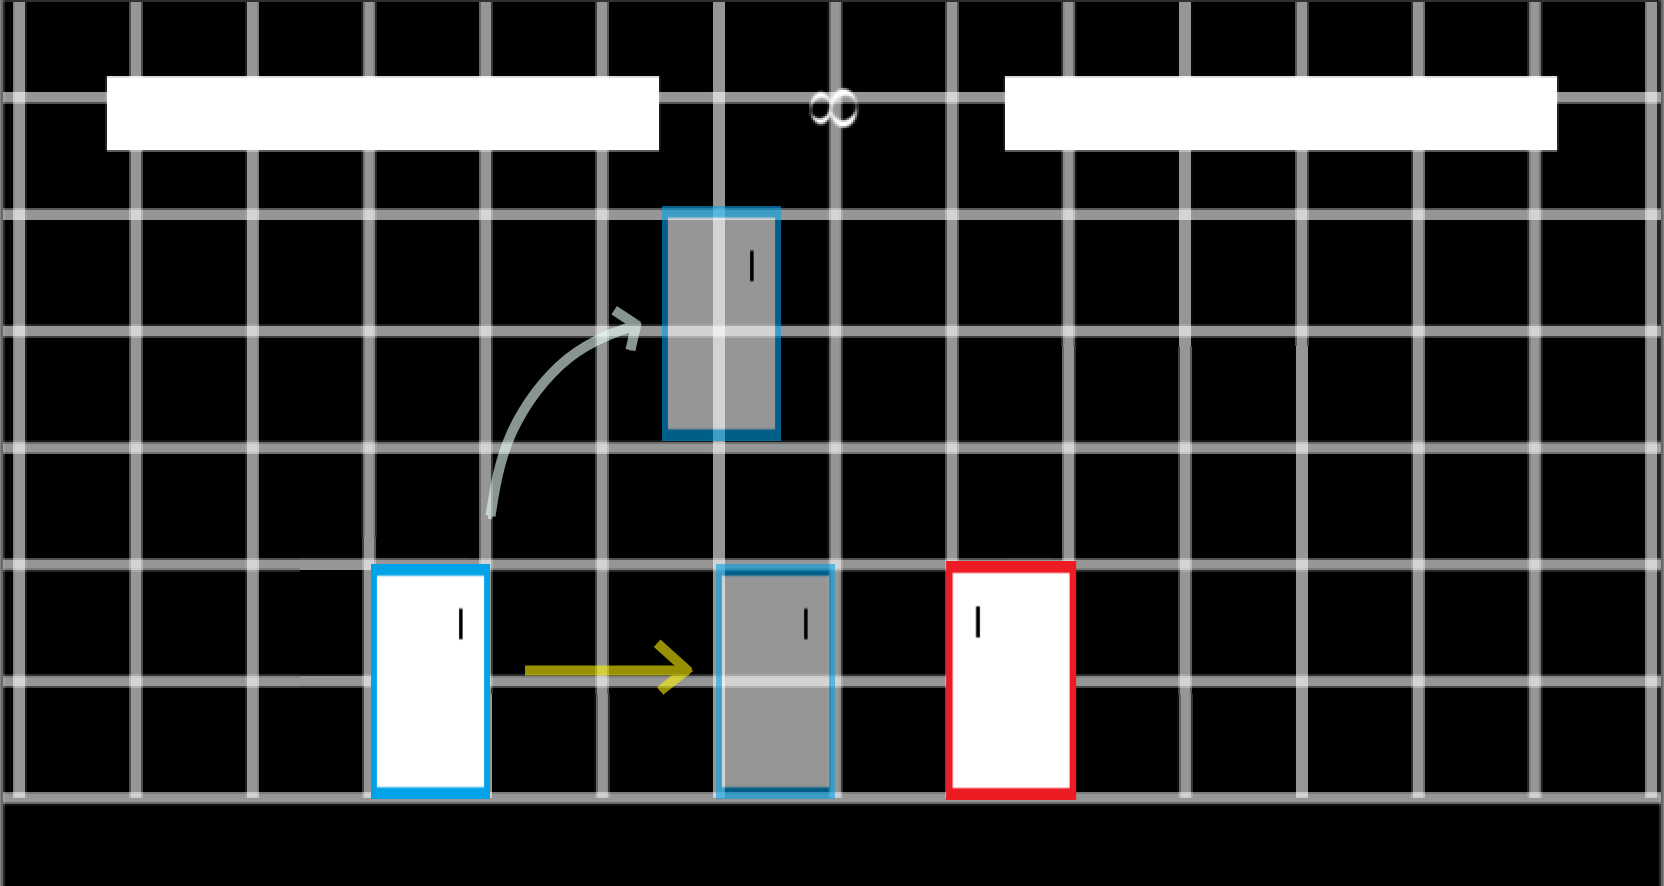
\includegraphics[width=\textwidth]{Figures/LearningExample1.png}
		\caption{Always doing the same action is too predictable}
		\label{Learning1}
	\end{subfigure}
	\begin{subfigure}[h]{0.4\textwidth}
		\centering
		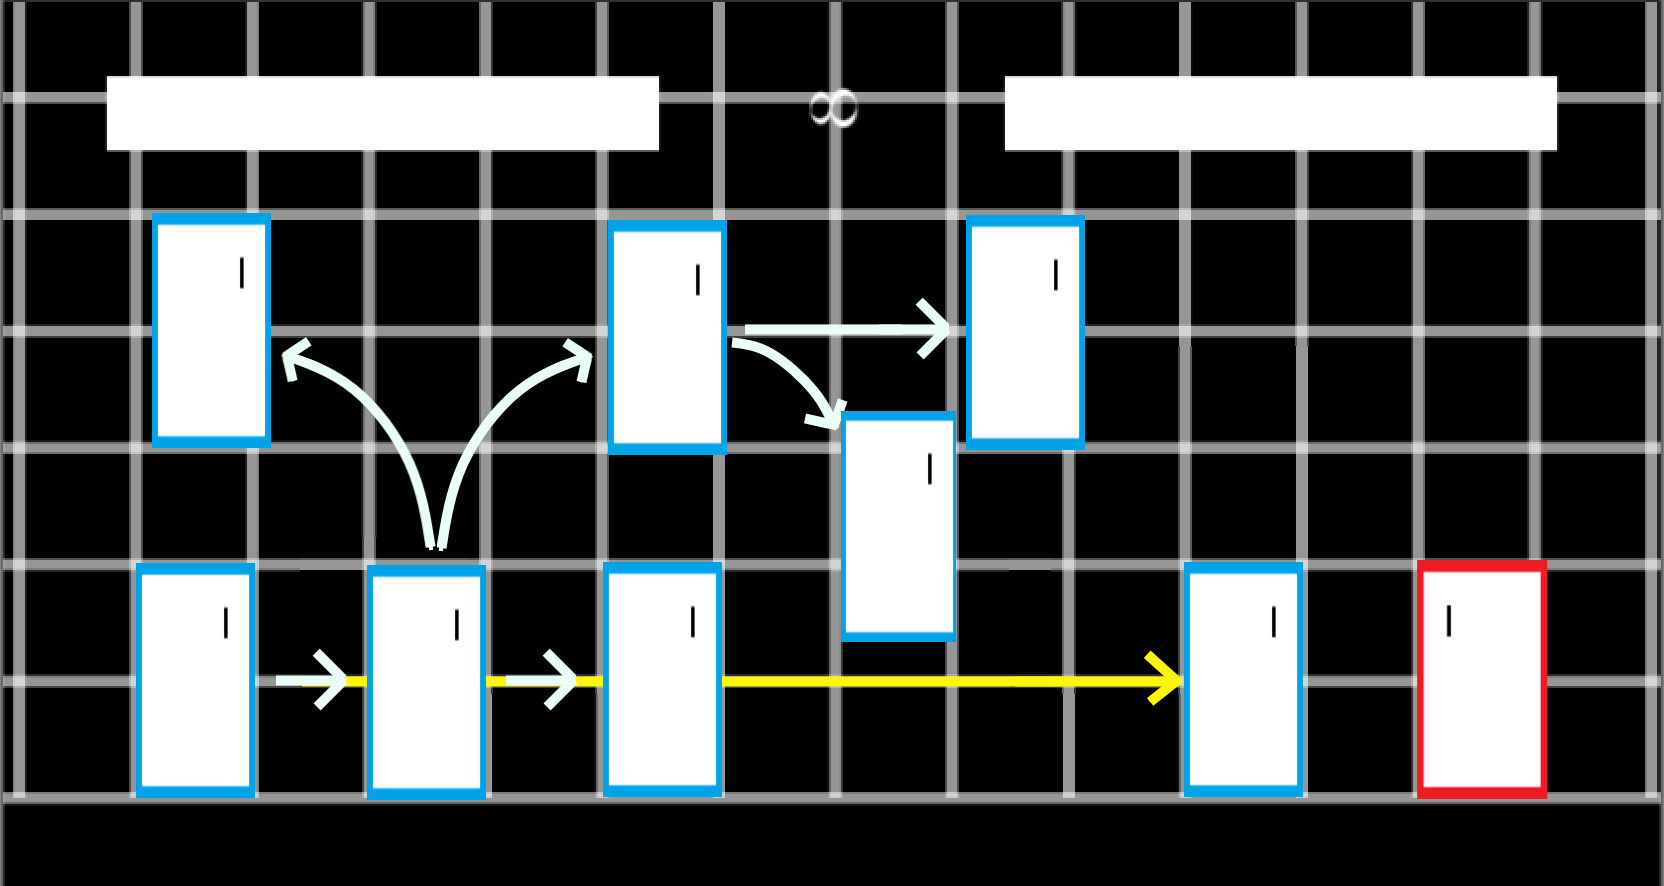
\includegraphics[width=\textwidth]{Figures/LearningExample2.png}
		\caption{Some actions don't make sense in the given context}
		\label{Learning2}
	\end{subfigure}
\end{figure}

%This is because while learning techniques are very good at determining the right move to make given a situation, they don't do a great job at planning long-term strategies. 

%Even if the algorithm learns the distribution of the actions that the player tends to take, a chain of selections would still be unlikely to form something that resembles cohesive strategy. This is because the AI has to decide on an action to perform on every frame. This ultimately results in the jittery movements that characterizes these kinds of AI's in dynamic environments, as it's hard for it to decide to do a single action for a prolonged period of time.

\section{Why Use Search?}

Because human-play is heavily predicated on the usage of different kinds of strategies, dynamically creating and executing the same strategies as the target player should mimic their playstyle quite well. Since strategies are essentially a sequence of actions that a player takes in order to arrive at a desired goal, the formulation of strategies can naturally be represented as a search problem over the state space. The target player's demonstrations can be used to inform the AI of the goals to target and the actions to use, and custom cost functions and heuristics can bias the search towards actions that closely mimic the player. In addition, the demonstrations can be used to create a model of the game state's dynamics, which would allow the AI to form cohesive plans even in unfamiliar starting states. 

To understand how an AI might effectively use search, consider the following kind of player behavior:

\begin{figure}[h]
	\centering
	\includegraphics[width=\textwidth]{Figures/Flowchart.png}
	\caption{Player Strategy Example}
	\label{Player Strategy}
\end{figure}

During the game, player 1 tends to try to stay within a certain range of the opponent and try to hit them with a low attack. If the opponent blocks the low attack, it sometimes then tries to jump in while the opponent can't move out of the way and hit them with a air attack. Essentially, player 1's behavior is composed of two strategies, one where they try to hit the opponent with a low attack and another where they force the opponent to try to block the air attack. We can easily identify the strategy that the player is currently executing by looking at the ultimate result that they are aiming for.

%In a learning context, the AI has to decide at each frame what action it must do. This means that as the AI is walking towards the opponent, it must decide at each frame that the correct action to do is walk left. However, this results in a series of issues on the implementation side. First of all, it requires that we must record the players action during every frame of a training episode, as otherwise unknown states would pop up all of the time as the player moves forwards. Further more, we quickly find that the AI performs poorly when starting in an unfamiliar position. This is because it is unlikely to find its way to a state that it has properly been trained on, and because it tries to pick an action to do at every frame, it is unlikely to reach a stable state and settle back into a correct strategy. Though function approximators can alleviate the tendency of the AI to take essentially random moves, it still is fairly ineffective at predicting the proper action in states that are unlike anything it's trained on. Though the initial demonstration can give the AI a pretty good idea of what to do when presented the exact same situation, it quickly falls apart the second we reach an unknown state. Compounded with the fact that we want to represent the game state with several categorical variables, this approach will likely fail to be robust enough to represent a human AI.

When the AI plans, it first determines what goal state to target. It then uses the actions pulled from the target player's demonstration and uses them to search the state space to reach the goal. For example, to reach the goal where the opponent is hit with a low attack, the search would return a plan where it walks forward to get close to the opponent, crouches, and then uses the low attack. If the opponent moves during that time, the AI replans picks a walking action that would put it in the correct range for hitting the opponent. With a single demonstration, search is able to formulate a plan that approximately resembles the strategy executed by the target player.

\section{Agent Framework Overview}

\begin{figure}[h]
	\centering
	\includegraphics[width=\textwidth]{Figures/SearchFlowChart.png}
	\caption{AI Framework}
	\label{transitions}
\end{figure}

The agent will work as follows. After taking in the game state, the agent forms a plan to reach a predefined goal state. The goal states are generated from the demonstration data, and the plan that the agent forms uses actions found in from the demonstration data. After producing the best available plan in the allotted amount of time, the agent then tries to execute that plan. After executing an action, it evaluates the game state. If the action brought the agent to the expected game state, it then will try to execute the next action in the plan. However, if the agent finds itself in an unexpected game state, it forms another plan to try to get to the goal. Once a plan is successfully executed or after enough time has passed, the agent picks a new goal state to target and repeats the process.


\chapter{Planning-based Approach in Details}

\label{Chapter4} % For referencing the chapter elsewhere, use \ref{Chapter1} 


\section{Action-$\delta$s}
First, we explain the concept of action-$\delta$s, which our work relies on. When a player takes action $a$ from state $s$ and arrives at state $s'$, the game state changes because of $a$. For example, the action of walking to the right causes the player's $x$-position to increase. We refer to this change in the game state as an action-$\delta$, which represents how the game state changes as a result of taking action $a$. Figure $\ref{action-d}$ shows that jumping to the right has an action-$\delta$ that puts the player up and to the right

\begin{figure}[h]
	\centering
	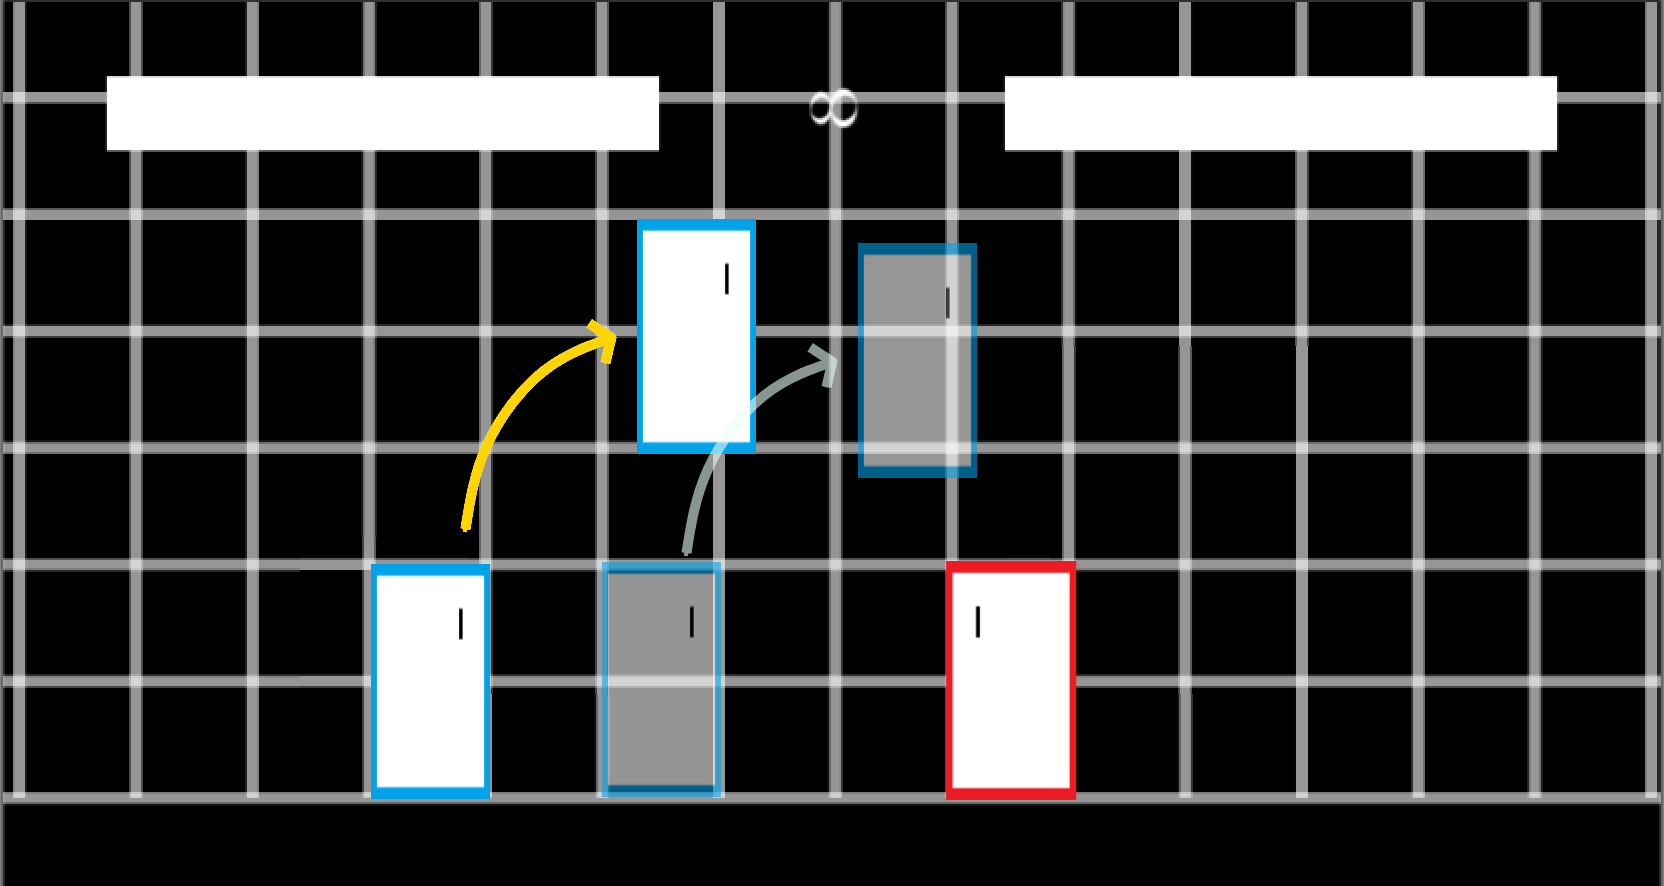
\includegraphics[width=\textwidth]{Figures/ActionDelta.png}
	\caption{Example Action-$\delta$}
	\label{action-d}
\end{figure}

These action-$\delta$s are used to understand and build a model of the game's dynamics. If we know how an action affects the game state in one situation, we can predict how the action will affect the game state in similar situation. 

\section{Demonstration $\delta$-Search}
The task of emulating a player's behavior is represented as a graph search problem. Specifically, the objective is to form a plan to hit the opponent using the actions demonstrated by the target player. The plan should be feasible and resemble a plan executed by the target player as much possible.

The search space is represented as graph $G = (V, E)$. The vertices $V$ of the graph are the various states of the game. The edges $E$ represent the possible transitions between game states. 

The transitions that we search on are generated from the training data and fall into two classes. The first class, known-transitions, are tuples $(s,a,s')$ which are identical to ones captured from the demonstration. The other class of transitions are referred to as $\delta$-transitions. These transitions are of the form $(s, a, \phi(s, a))$, where $\phi(s, a)$ is a predictor function that takes in the current state $s$ and an action $a$ performed by the target player. This predictor function generates the predictions by learning from the action-$\delta$s of action $a$ that were obtained from the training data.

Since we want to form a plan that hits the opponent, a valid goal state is one where the opponent has the "FirstHit" status. During a run of the search, the goal is defined to be a state that has the same characteristics as a goal state selected from the demonstration. The goal state is selected according to a weighted distribution. This ensures that the planner's ultimate objective matches that of the target player.

When searching for a feasible plan to get to the goal, we use a modified version of heuristic graph search. We maintain two priority queues throughout the search, one called KNOWN and another called UNKNOWN. When deciding to expand a state, we prioritize expanding states in KNOWN. These states are states which have been seen in the demonstration, which allows us to use the known-transitions to generate the successor states. If there are no states in KNOWN, then we expand states from UNKNOWN using the $\delta$-transitions. After expanding a state, all successors states which have not been expanded by $\delta$-transitions are added to the UNKNOWN priority queue. If a state has been seen in the demonstration and it has not yet been expanded by known-transitions, it is added to the KNOWN priority queue. Once we find a state that is a goal state, we return the plan to that state.

Prioritizing known-transitions makes it so that the plan we form tries to use actions shown in the demonstration as much as possible. This is a desirable quality as replicating the demonstrated actions in the proper situations precisely replicates that human's behavior in those instances. It also has the effect of reducing the number successors we add to our priority queues, which is important as the number of $\delta$-transitions increases with the number of unique actions in our demonstration data set.

Pseudo-code for this algorithm can be found in Section 4.8.

\begin{figure}[t]
	\centering
	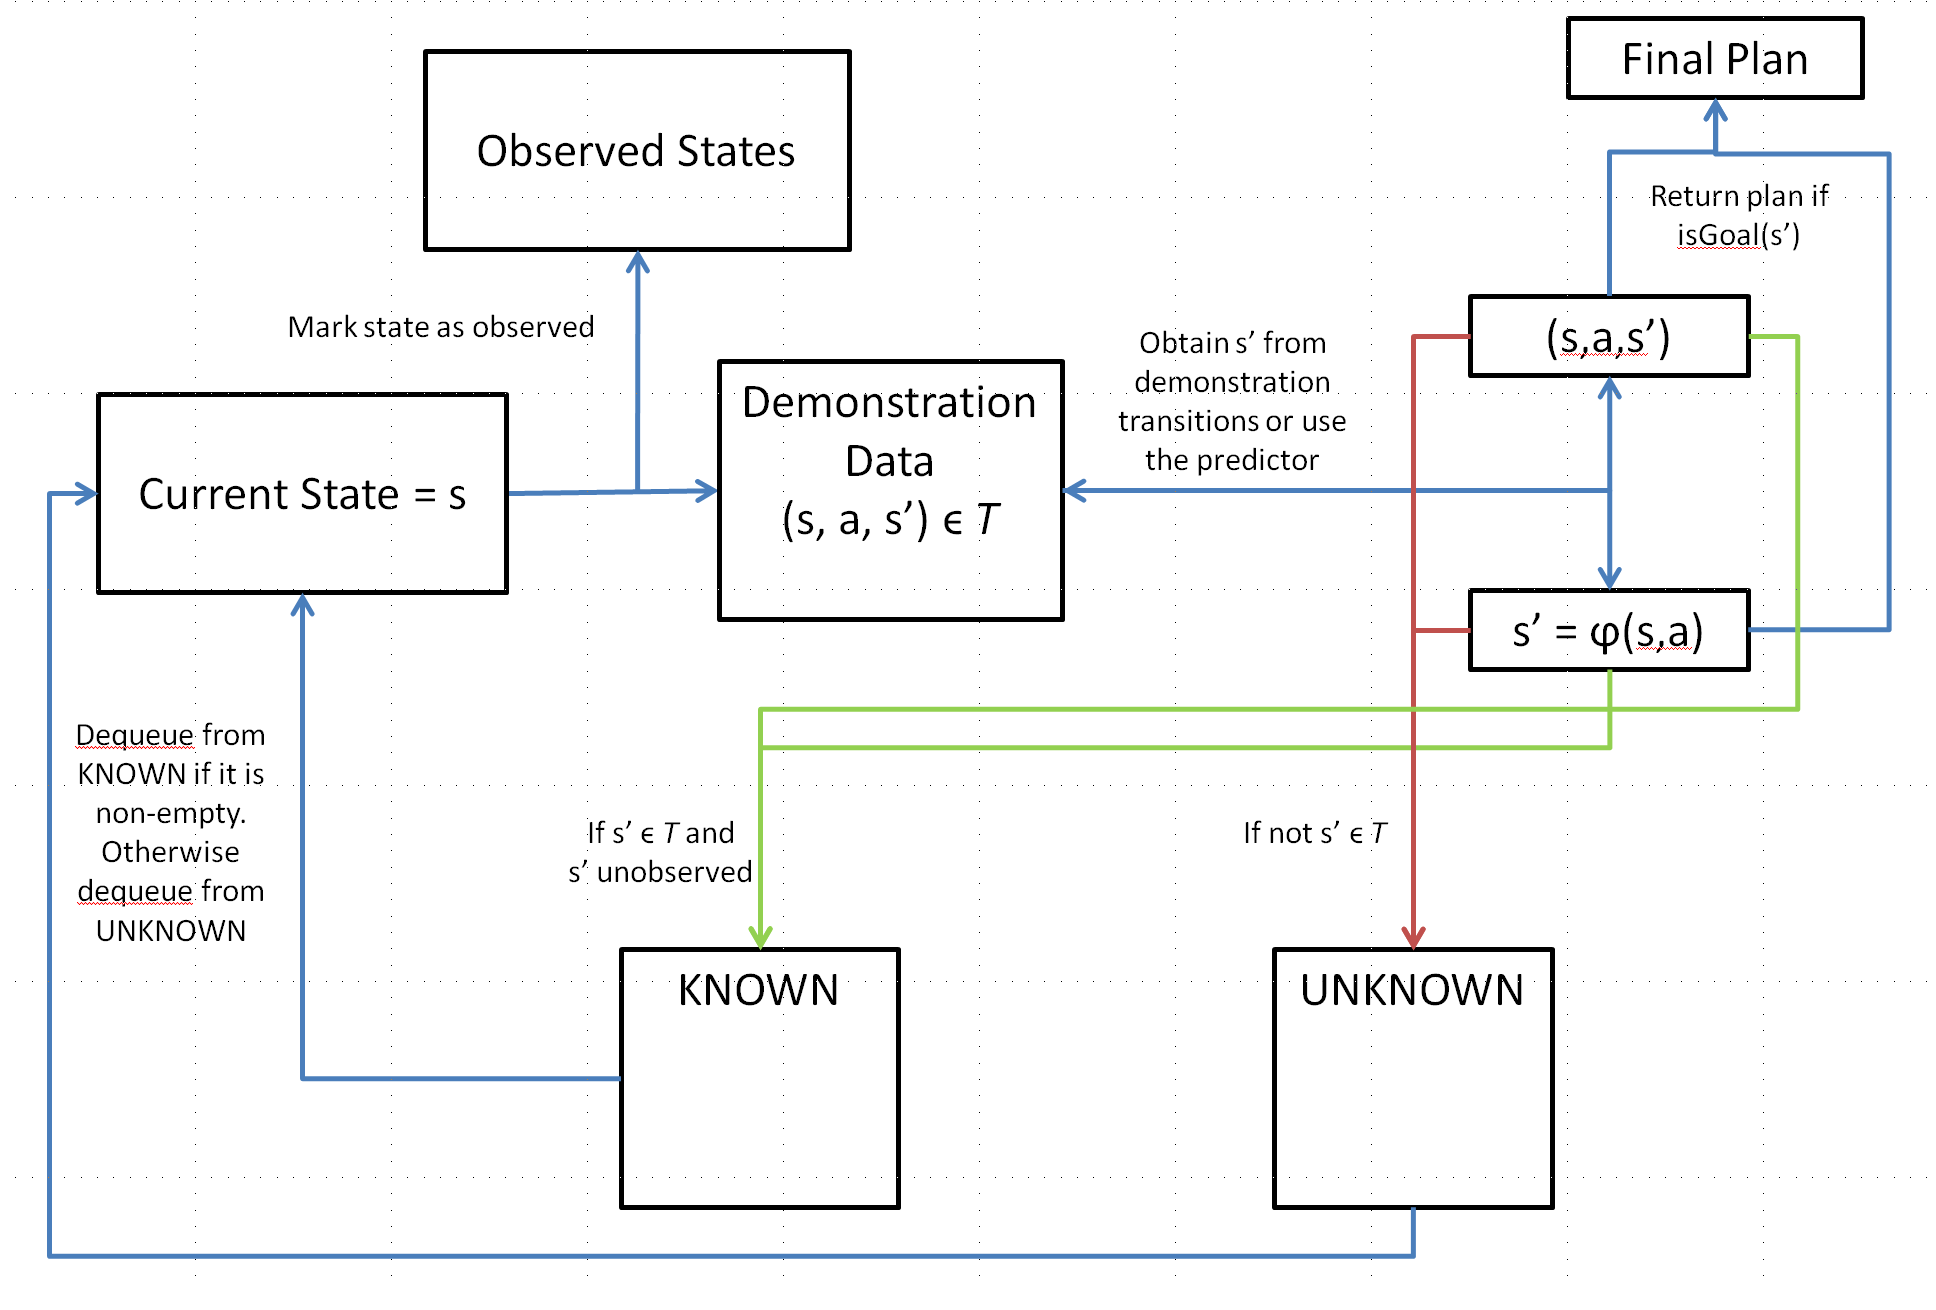
\includegraphics[width=\textwidth]{Figures/SearchSpecificFlowchart.png}
	\caption{Overview of $\delta$-search}
	\label{}
\end{figure}

\section{Environment Description}
The environment used to test this approach is a fighting game we created called \textit{FG}. This gave us complete control over the dynamics of the game. It also gave us access to internal game data which would have been considerably more difficult to access had we instead opted to modify an existing fighting game. 

The game is structured as a traditional fighting game. Players move back and forth on in a 2D space, trying to land blows on one another to reduce the opponent's health to zero. There are a total of 21 types of actions that the player can perform, and each of these actions can be done for a duration that corresponds to some number of frames. The specific types of actions that players can take are described in Table \ref{actions}.

The state of the game is represented by a combination of the states of the player and opponent. A player's state includes its world position in discretized space, an indicator of its velocity, and its current status. Details are described in Table \ref{gamestate} and Table \ref{playerstatus}




%Old Stuff from Previous Drafts
%In order to perform search, we need a way to generate the successors of state $s$. Specifically, we need a way to generate $s' = succ(s, a)$ where $a$ is an action defined by a type and a duration. Because we don't actually know the full dynamics of the game, we extract them from the player's demonstration.


%An issue that still is prevalent is that of robustness. When the AI encounters a state that it hasn't seen before, what should it do? We propose to solve this issue using a technique we dub \textbf{action effects}. The idea is that many actions have easily predictable actions. For example, moving left for a long time will always move the player a certain distance to the left. This formulation works for this domain because the results of actions in fighting games are completely predictable, as it's all codified inside the game engine. 

%What does one do with these action effects? Well, we can use them to give the AI an idea of what to do in a state it hasn't seen before

%\begin{figure}[t]
%	\centering
%	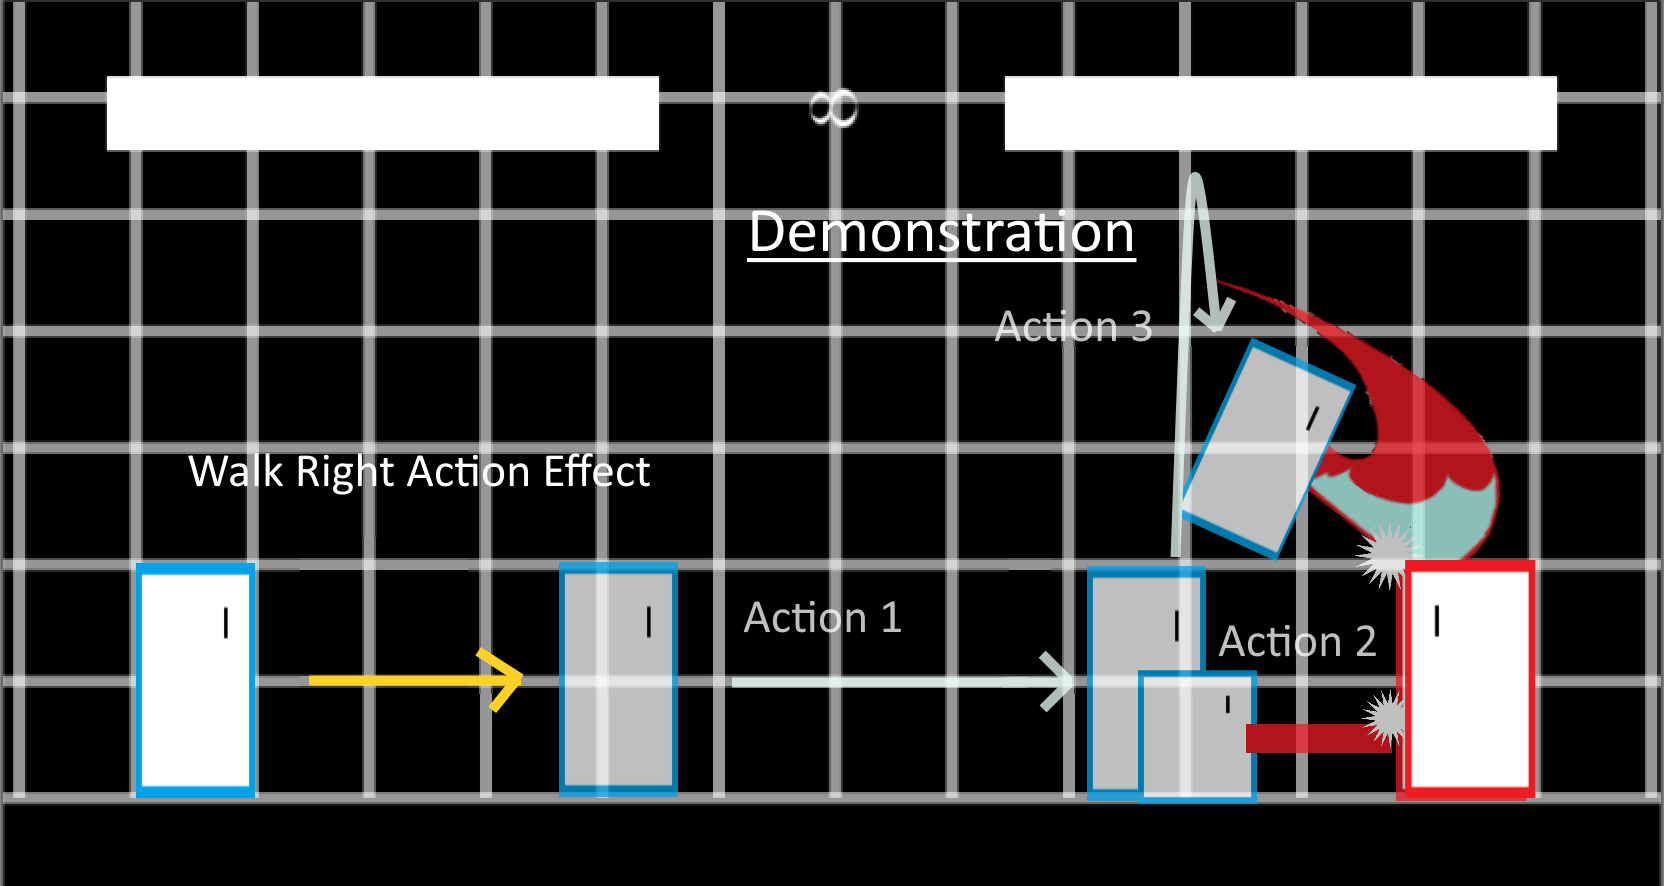
\includegraphics[width=\textwidth]{Figures/ActionEffect.png}
%	\caption{Action Effects}
%	\label{ActionEffects}
%\end{figure}


%For example, lets say that the player starts from far away from the demonstration etc etc.


%\section{Algorithm Design and implementation}

%In order to formulate the fighting game as a search problem, we need to discretize the state space as a graph. The nodes on this graph represent the game state at a specific point in time. This includes the positions of the players, their velocities, and various other metrics that capture their internal state. Full details can be found in Table \ref{gamestate}. The edges between nodes $a$ and $b$ represent transitioning from state $a$ to state $b$ via a \textbf{preformed action}. These are tuples which dictate an \textbf{type} of action that a player can perform and a \textbf{duration} that it is performed for. The set of actions that the AI can perform is restricted to the actions performed by the player in the training data. 

%\subsection{Extracting game dynamics}

\section{Extracting Data from Demonstrations}

In order for the AI to generate plans, we need a human demonstration to build a model of the game dynamics. Throughout this section, we will refer to a simple human demonstration where the player moves forward, hits the opponent with a low attack, and then jumps to hit the player with a jumping attack.

\begin{figure}[h]
	\centering
	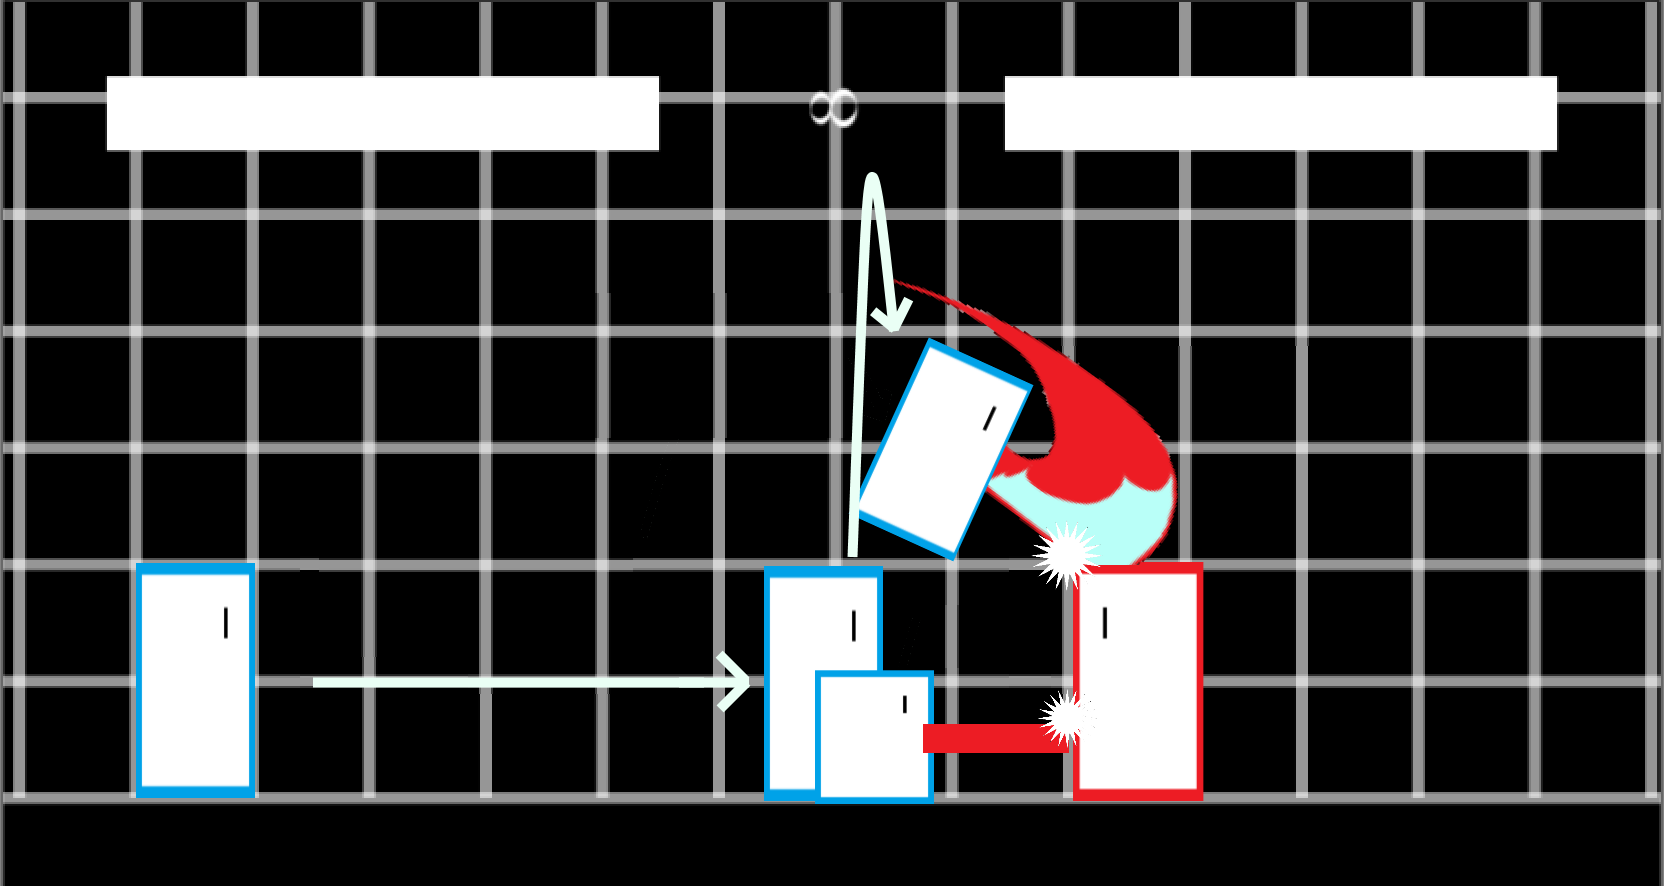
\includegraphics[scale=0.5]{Figures/Demonstration.png}
	\caption{Example of a Human Demonstration}
	\label{ActionEffects}
\end{figure}

As the demonstration plays out, the target player performs actions to transition between different game states. A transition $(s,a,s')$ is recorded in each of the following cases

1. When the player starts performing a new action

2. When the player is hit during the current action, ending it early. 

3. When the game state changes during the current action.

\begin{figure}[h]
	\centering
	\begin{subfigure}[h]{0.3\textwidth}
		\centering
		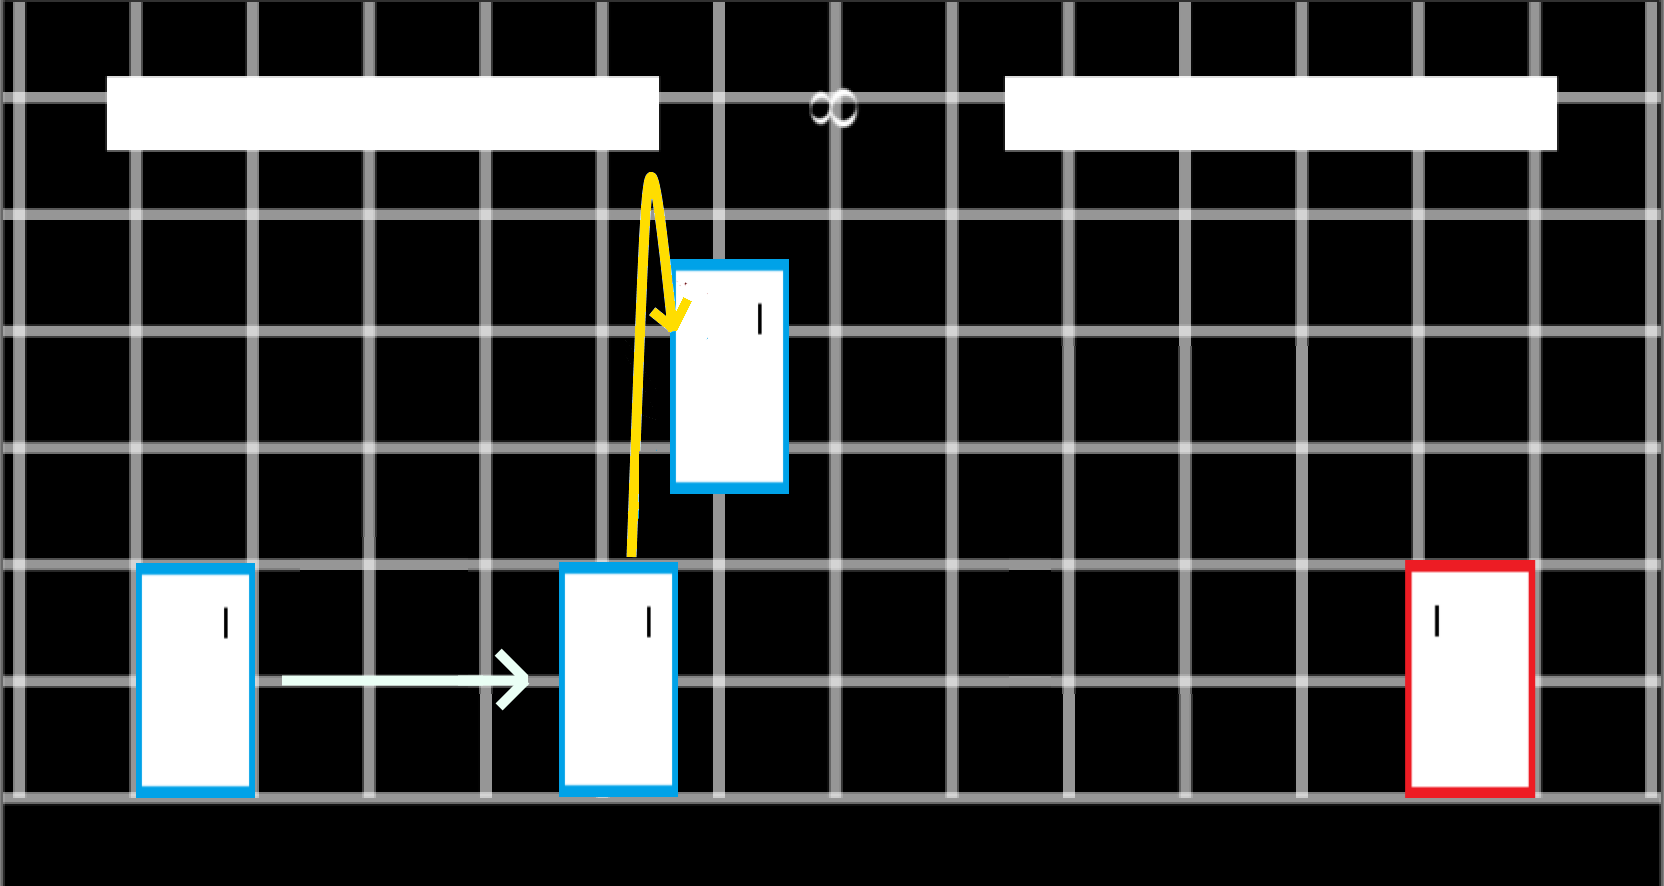
\includegraphics[width=\textwidth]{Figures/Example1.png}
		\caption{case 1}
		\label{}
	\end{subfigure}
	\begin{subfigure}[h]{0.3\textwidth}
		\centering
		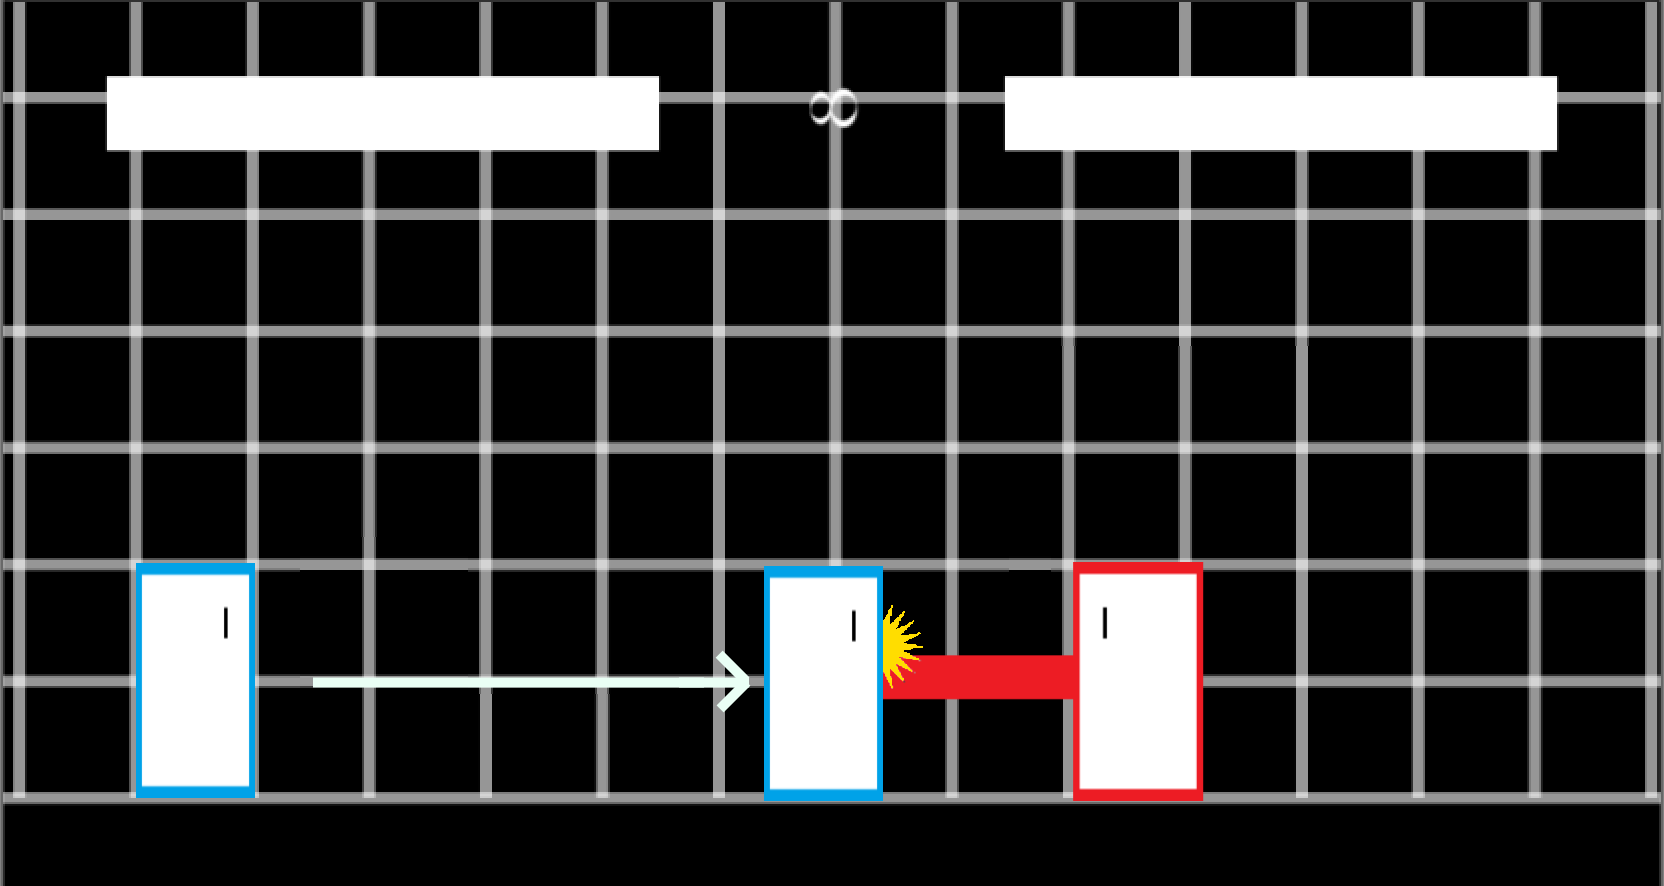
\includegraphics[width=\textwidth]{Figures/Example2.png}
		\caption{case 2}
		\label{}
	\end{subfigure}
	\begin{subfigure}[h]{0.3\textwidth}
		\centering
		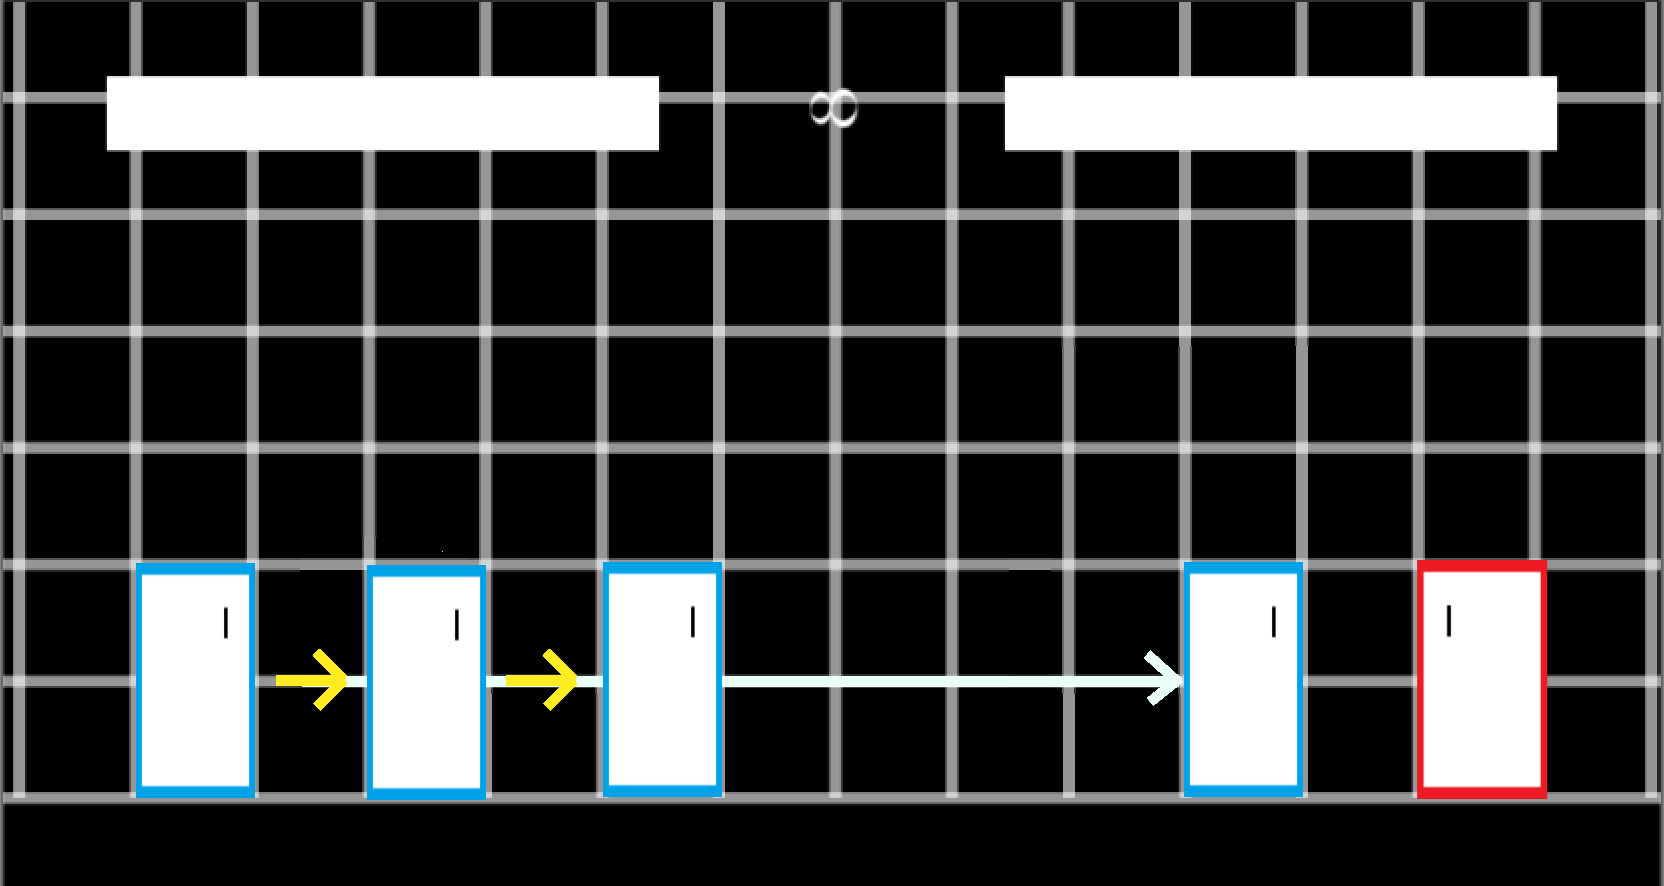
\includegraphics[width=\textwidth]{Figures/Example3.png}
		\caption{case 3}
		\label{}
	\end{subfigure}
\end{figure}

The last case is particularly important for the algorithm, as it breaks down the single player's action of walking forward into multiple smaller component actions that the AI can use.

These transitions are saved as both known-transitions and $\delta$-transitions. All known transitions are stored in a table $K$ where $K[s]$ contains a list of all outgoing transitions $(a,s')$. All $\delta$-transitions are also saved into a table $D$ where $D[a]$ contains all action-$\delta$s encountered. 

An action-$\delta$ is calculated as follows given an observed transition $(s, a, s')$. $p$ represents the target player's state information an $q$ represents the opponent's state information

\begin{table}[h]
	\centering
	\caption{How Action-$\delta$ is Calculated}
	\begin{tabular}{| c | c | c | c |}
		\hline
		 & $s$ & $s'$ & action-$\delta$ \\
		\hline
		x Position        			& $p_{x}$ & $p_{x}'$ & $p_{x}' - p_{x}$ 	\\
		\hline            			
		y Position        			& $p_{y}$ & $p_{y}'$ & $p_{y}' - p_{y}$ 	\\
		\hline            			
		x Velocity        			& $p_{xVel}$ & $p_{xVel}'$ & $p_{xVel}' - p_{xVel}$  \\
		\hline            			
		y Velocity        			& $p_{yVel}$ & $p_{yVel}'$ & $p_{yVel}' - p_{yVel}$	\\
		\hline
		opponents x Position        & $q_{x}$ & $q_{x}'$ & $q_{x}' - q_{x}$	\\
		\hline
		opponents y Position        & $q_{y}$ & $q_{y}'$ & $q_{y}' - q_{y}$ \\
		\hline
		opponents x Velocity        & $q_{xVel}$& $q_{xVel}$' & $q_{xVel}' - q_{xVel}$	\\
		\hline
		opponents y Velocity        & $q_{yVel}$ & $q_{yVel}'$ & $q_{yVel}' - q_{yVel}$	\\
		\hline
		grounded        			& $p_{grounded}$ & $p_{grounded}'$ & $p_{grounded}'$	\\
		\hline
		opponent grounded       	& $q_{grounded}$ & $q_{grounded}'$ & $q_{grounded}'$ 	\\
		\hline
		status       				& $p_{status}$ & $p_{status}'$ & $p_{status}'$ 	\\
		\hline
		opponents status        	& $q_{status}$ & $q_{status}'$ & $q_{status}'$ 	\\
		\hline
	\end{tabular}
	\label{gamestate}
\end{table}

In the case of the simple demonstration, some of the known-transitions that are extracted are found in Table $\ref{known-transitions}$

\begin{table}[h]
	\centering
	\small
	\begin{tabular}{| c | c | c |}
		\hline
		s & a & s' \\
		\hline
		[-6,0,0,0,1,0,0,0,true,true,Stand,Stand] & WalkRight 1 & [-6,0,1,0,1,0,0,0,true,true,Moving,Stand]\\
		\hline
		[-6,0,0,0,1,0,0,0,true,true,Stand,Stand] & WalkRight 10 & [-4,0,1,0,1,0,0,0,true,true,Moving,Stand]\\
		\hline
		[-6,0,0,0,1,0,0,0,true,true,Stand,Stand] & WalkRight 30 & [0,0,1,0,1,0,0,0,true,true,Moving,Stand]\\
		\hline
		[0,0,1,0,1,0,0,0,true,true,Moving,Stand] & Crouch 1 & [0,0,0,0,1,0,0,0,true,true,Crouch,Stand]\\
		\hline
		[0,0,1,0,1,0,0,0,true,true,Crouch,Stand] & JumpNeutral 1 & [0,0,0,1,1,0,0,0,false,true,Air,Stand]\\
		\hline
		[0,0,1,0,1,0,0,0,true,true,Crouch,Stand] & JumpNeutral 45 & [0,0,0,-1,1,0,0,0,false,true,Air,Stand]\\
		\hline
		[0,0,0,-1,1,0,0,0,false,true,Air,Stand] & AirAttack 3 & [0,0,0,-1,1,0,0,0,false,true,AirAttack,FresHit]\\
		\hline
	\end{tabular}
	\caption{Demonstration Known-Transitions}
	\label{known-transitions}
\end{table}

\newpage

The corresponding action-$\delta$s are then described in Table $\ref{delta-transitions}$

\begin{table}[h]
	\centering
	\begin{tabular}{| c | c |}
		\hline
		a & action-$\delta$ \\
		\hline
		WalkRight 1 & [0,0,1,0,0,0,0,0,true,true,Moving,Stand]\\
		\hline
		WalkRight 10 & [2,0,1,0,0,0,0,0,true,true,Moving,Stand]\\
		\hline
		WalkRight 30 & [6,0,1,0,0,0,0,0,true,true,Moving,Stand]\\
		\hline
		Crouch 1 & [0,0,0,0,0,0,0,0,true,true,Crouch,Stand]\\
		\hline
		JumpNeutral 1 & [0,0,0,1,0,0,0,0,true,false,Air,Stand]\\
		\hline
		JumpNeutral 45 & [0,0,0,-1,0,0,0,0,false,true,Air,Stand]\\
		\hline
		Attack 3 & [0,0,0,-1,1,0,0,0,false,true,AirAttack,Freshit]\\
		\hline
	\end{tabular}
	\caption{Demonstration Action-$\delta$s}
	\label{delta-transitions}
\end{table}

Lastly, we extract goal-states from the demonstration. These are simply states $s'$ found from the transitions where the opponent's status is \textit{FreshHit}. The set of goal states obtained from the demonstration are seen in Table $\ref{goalstates}$

\begin{table}[h]
	\centering
	\begin{tabular}{| c | c | c | c | c | c | c | c | c | c | c | c |}
		\hline
		$p_x$ & $p_y$ & $p_{xVel}$ & $p_{yVel}$ & $q_x$ & $q_y$ & $q_{xVel}$ & $q_{yVel}$ & $p_{grounded}$ & $q_{grounded}$ & $p_{status}$ & $q_{status}$\\
		\hline
		0 & 0 & 0 & 0 & 0 & 0 & 0 & 0 & true & true & LowAttack & FreshHit\\
		\hline
		0 & 0 & 0 & -1 & 1 & 0 & 0 & 0 & false & true & AirAttack & FreshHit\\
		\hline
	\end{tabular}
	\caption{Demonstration Goal States}
	\label{goalstates}
\end{table}


\section{Generating Successors}

When trying to figure out the successor of a state-action pair $(s,a)$, we have either seen that tuple in the demonstration or we haven't. If we have, we can generate the successor using a known-transition. The resulting successor is the same $s'$ as the one observed in the demonstration transition $(s,a,s')$. By traveling along known-successors, the plan generated by the search closely follows the exact actions taken by the player during demonstration

%\begin{figure}[h]
%	\centering
%	
\includegraphics[width=\textwidth]{Figures/Placeholder.png}
%	\caption{The AI follows the player's demonstration}
%	\label{followdemonstration}
%\end{figure}

If $(s,a)$ has not been seen in the demonstration data, then we have to use a $\delta$-transition. When generating a successor using $\delta$-transitions, we rely on a predictor function $\phi(s,a)$. The predictor works as follows.

To determine the effect of taking action $a$, we look at all action-$\delta$s associated with action $a$. We will refer to these action-$\delta$s as $\delta$. Each $\delta$ has a \textit{prior} called $s_{\delta}$, which indicates the starting state of that particular recorded transition. We can assign a similarity score between the $s$ and $s_{\delta}$, which we use as a rough approximation of our confidence in the truth of that action.

$$sim(s, s_{\delta}) = 1-\frac{\sum_i dist(s[i], s_{\delta}[i])}{\sum_i max_i}$$

$$dist(s[i], s_{\delta}[i]) =
\begin{cases}
s_{\delta}[i] - s[i] & \text{if $i$ represents the x position of either player} \\
s_{\delta}[i] == s[i] & \text{otherwise}
\end{cases}
$$

$s[i]$ represents the value of field $i$ in state $s$ and $max_[i]$ represents the maximum value of $dist(s[i], s_{\delta}[i])$. 

We then create a predicted action-$\delta$ by taking a weighted average over the action-$\delta$s and the similarity score and then rounding the result.

$$\delta^*[i] \approx
\begin{cases}
argmax_\delta \frac{sim(s, s_{\delta})}{\sum_\delta sim(s, s_{\delta})}[i] & \text{if $s[i]$ is a categorical variable} \\
\sum_\delta \frac{sim(s, s_{\delta}) \delta[i] }{\sum_\delta sim(s, s_{\delta})} & \text{otherwise}
\end{cases}
$$

To get the final prediction, we apply $\delta^*$ to the current state $s$ to get $s'$. For categorical variables, $s'[i] = \delta*[i]$ and for everything else, $s'[i] = s[i] + \delta*[i]$

The confidence value $c$ that is returned with this prediction is calculated as follows.

$$c = sim(s, s_{\delta}) \text{ where } \delta = argmax_\delta \frac{sim(s, s_{\delta})}{\sum_\delta sim(s, s_{\delta})}$$

This represents our belief in the predicted result and it also gives an indication of likelihood that the player would take this action.

%With the model of the game dynamics, we can then begin to compute the successors of state $s$. There are two cases that we differentiate between.

%\textbf{Case 1: Known states}
%If $s$ is a state that was encountered in the demonstration, then we have precise knowledge of the player's behavior in that state. Specifically, $T[s]$ contains all of actions $A$ that the player has taken at that state. To best model the player the AI restricts itself to taking the same kinds of actions that the player has in those states, so it only adds $succ(s,a)$ where $a \in A$. In addition, we have good predictions for the value of $s' = succ(s,a)$ since we have the transitions $(s,a,s')$ stored within $T$.

%==========Insert example of the simple look up here============

%\textbf{Case 2: Unknown states}
%The AI is likely to see states which were not seen during the demonstration. In this case, we have no clear basis for knowing what the target player would do. 

%In this case, we first determine the types of actions that are valid in the AI's current state. This rules out using impossible actions, such as walking forward while the AI is airborne. From the remaining action types, we look at all valid actions $a$ from the demonstration and predict the result of taking that action.

%Specifically, the predictor is works as follows. To determine the effect of taking performed action $a$, we look at $D[a]$. We then do a weighted average over all of $\Delta_a$ to derive the final prediction. The weighting is set according to the similarities of the prior states for each action effect.

\section{Costs}

In order to differentiate the qualities of plans, we need a suitable cost function. The cost of taking a known-transition is 1.0, as there is no qualitative way to evaluate one demonstrated action as being more "human-like" than another. For a $\delta$-transitions, we apply an additional penalty that is inversely proportional to the confidence returned by the predictor.\\

$$(s',c) = \phi(s, a)$$
$$Cost(s, s') = \lambda/c$$

Where $\lambda$ is a hypervariable. This makes it so that shorter plans which use higher confidence transitions are favored. 

\section{The Goal and Heuristics}

Before beginning the search, we select a random goal state from the demonstration to target. This the goal states selected are weighted by their similarity to the initial starting state. Goals are selected randomly because it simulates how a player might vary its objective during gameplay. This goal state has certain qualities that are important to target. Namely, we care about the distance between the player and the opponent and the statuses of the player and opponent. The search tries form a plan that results in a state which matches these qualities, shown in Table $\ref{qualities}$. 

\begin{table}[h]
	\centering
	\caption{Qualities Extracted from State $s$}
	\begin{tabular}{| c | c | c | c |}
		\hline
		Field Name & Value\\
		\hline
		x Distance        			& $|p_x - q_x|$ \\
		\hline            			
		y Distance        			& $|p_y - q_y|$ 	\\
		\hline
		grounded        			& $p_{grounded}$ \\
		\hline
		opponent grounded       	& $q_{grounded}$ \\
		\hline
		status       				& $p_{status}$ \\
		\hline
		opponents status        	& $q_{status}$ \\
		\hline
	\end{tabular}
	\label{qualities}
\end{table}

In order to efficiently guide the search towards such a state, we reduce the current state to these qualities. The heuristic we use is then a measure the total distance between the current state's qualities and the goal state's qualities. The quality of a state is shown in the below table.



%\section{Goal states and Heuristics}
%The final component we need to effectively perform search in this space is a goal state and heuristic function. 

%Because our objective is to have the AI exhibit a certain kind of behavior, the goal state is only partially-specified. The function \textit{IsGoal()} determines whether a state is a goal state and is designed as follows.

%Firstly, because this AI is intended to provide competitive players an more authentic representation of human play, the considered state must have the opponent in the \textit{FirstHit} status. Additionally, human players mix up their short-term strategies for getting hits so that they aren't predictable. To emulate this characteristic, we randomly select an instance in our demonstration where the opponent has the \textit{FirstHit} status and designate that as the \textbf{target}. We then require that the considered state has qualities similar to the target. This refers to the relative positions of the players and characteristics of each player's behavior states. 

%For the heuristic, when evaluating state $s$, we took the Manhattan Distance of the relative positions of the 2 players and added that to the number of other parameters in $s$ which do not match the values in the target state $t$.

%This \textbf{IsGoal()} function and the heuristic then gives us the following kind of behavior.

%\begin{figure}[t]
%	\centering
%	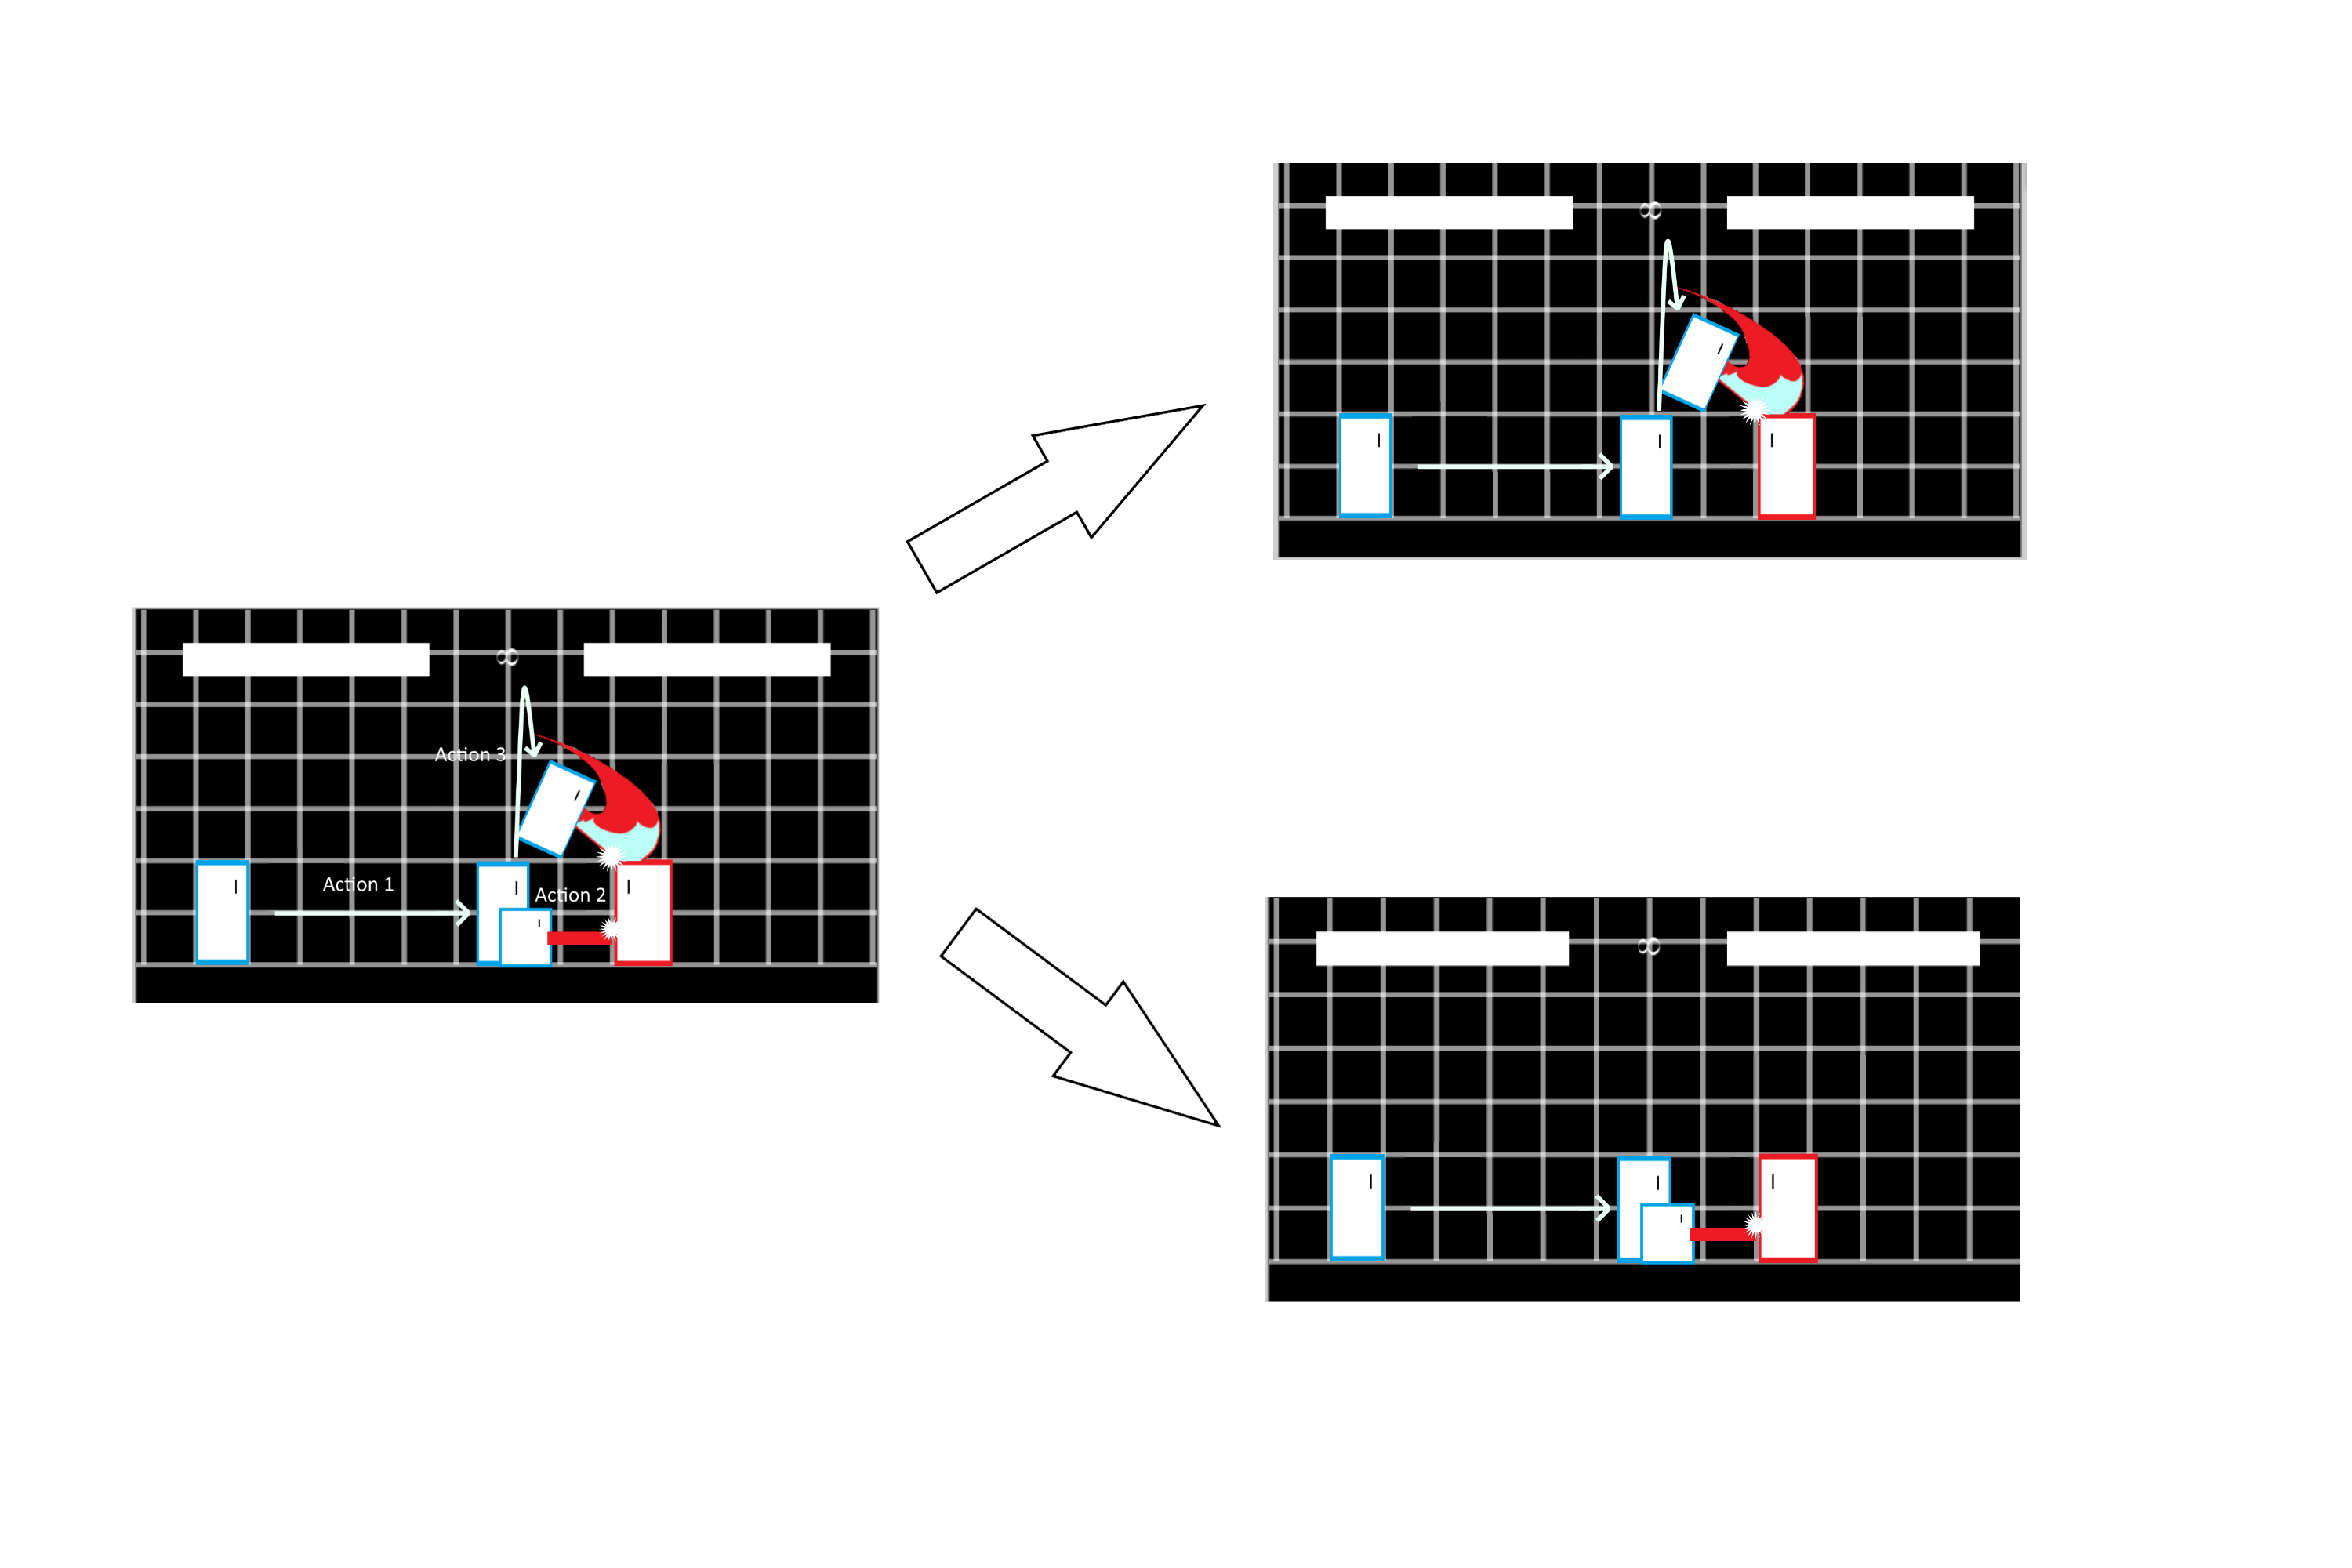
\includegraphics[width=\textwidth]{Figures/DecisionMaking.png}
%	\caption{Action Effects}
%	\label{ActionEffects}
%\end{figure}

%In the demonstration, we have one instance where the player hits the opponent with a low attack and another instance where the player hits the opponent with a jumping attack. One of the instances is randomly selected to be the target, and the AI then follows the appropriate plan to execute.

\newpage
\section{Pseudo-Code}

\begin{algorithm}
	\begin{algorithmic}[1]
		\Function{$\delta$-search($s_{start}, demonstrations$)} {}
		\State $OBS = \{\}$
		\State $OBS_{\delta} = \{\}$
		\State $KNOWN = \{\}$
		\State $UNKNOWN = \{\}$
		\State $s_{goal} = GetGoal(demonstrations)$
		\State $KNOWN \cup \{s_{start}\}$, $UNKNOWN \cup \{s_{start}\}$
		\While {$|KNOWN| \not = 0$ OR $|UNKNOWN| \not = 0$}:
		\If {$|KNOWN| \not = 0$}
		\State Remove the smallest $[f(s) = g(s) + h(s)]$ from $KNOWN$
		\State $OBS \cup \{s\}$
		\If {$isGoal(s)$}	return $plan(s)$ 
		\EndIf
		\State Expand $s$ with $(s,a,s') \in demonstrations$ \hfill $s' \not \in OBS$ OR $s' \not \in OBS_{\delta}$
		\If {$(s', \_, \_) \in demonstrations$}
		\State $KNOWN \cup \{s'\}$
		\EndIf
		\State $UNKNOWN \cup \{s'\}$
		\ElsIf{$|UNKNOWN| \not = 0$}
		\State Remove the smallest $[f(s) = g(s) + h(s)]$ from $UNKNOWN$
		\If {$isGoal(s)$}	return $plan(s)$
		\EndIf
		\State $OBS_{\delta} \cup \{s\}$
		\State Expand $s$ with $s' = \phi(s,a)$ \hspace{2cm}  $s' \not \in OBS$ OR $s' \not \in OBS_{\delta}$
		\If {$(s', \_, \_) \in demonstrations$}
		\State $KNOWN \cup \{s'\}$
		\EndIf
		\State $UNKNOWN \cup \{s'\}$	
		\EndIf
		\EndWhile
		\EndFunction
	\end{algorithmic}
	\caption{Full Pseudo-Code of $\delta$-search}
\end{algorithm}

\section{Additional Considerations}

\subsection{Dealing with Long Search Times: Real-time Search}
Because of fast-paced nature of fighting games, players need to be able to reliably make split second decisions. This constraint then extends to our AI, as it can't afford to plan seconds at a time, as the game state might change drastically within that time period. In our implementation, the AI is required to come up with a plan within 50 milliseconds. If it cannot reach a goal state, it instead formulates a plan to get to an explored state which is the most similar to the current goal state. The idea is that by reaching this intermediate state, it can then resume planning from the position that is closer to the goal, giving the impression of one seamless plan, when it in fact generated that plan during execution.

%\begin{figure}[h]
%	\centering
%	
\includegraphics[width=\textwidth]{Figures/Placeholder.png}
%	\caption{The AI finds the best available state}
%	\label{anytime}
%\end{figure}

\subsection{Dealing with a Changing Game State: Replanning}
Because the opponent is allowed to move during plan execution, the plan we formulate is likely to encounter states which do not match the planned transitions. Because of the short time to plan we enforced, we can seamlessly replan whenever we hit an unexpected state and have the AI adjust accordingly. An example of this is when the opponent moves back while the AI is approaching them. Due to replanning, the AI will then know to continue to move towards the opponent, rather than stopping at its original location and attacking like initially planned.

%\begin{figure}[h]
%	\centering
%	
\includegraphics[width=\textwidth]{Figures/Placeholder.png}
%	\caption{The AI quickly forms a new plan}
%	\label{replanning}
%\end{figure}

\subsection{Dealing with Bad Predictions, Updating the Predictor}
One final thing that we do to ensure that our AI is robust is update the predictor. As the game progresses, the AI logs the transitions that don't match up with its predictions and adds it back to the training set. This helps the AI make better predictions in the future and helps avoid local minima plans. This is crucially important as otherwise the AI is likely to get stuck performing the same action repeatedly.


%\section{Justification and Objectives}
 
%
\chapter{Results and Discussion}

\label{Chapter5} % For referencing the chapter elsewhere, use \ref{Chapter1} 

\section{Results}

To test the AI's performance, we set up the following experiment. First, the subject was given time to familiarize and acclimate themselves to the controls and dynamics of the game. Afterwards, the subject played five 20 second long matches against a computer opponent that follows a set defensive behavior pattern. A random set of matches from this pool was selected to be the demonstration sessions, while the rest were grouped into a set of holdout sessions. We then used the data from the demonstration session to create three kinds of agents. One of the agents used our novel search technique. We refer to this agent as Search AI. The other agents implemented an simple N-gram AI and the adaptive Ghost AI and served as a point of comparison. An N-gram AI is essentially a vanilla GhostAI that is not aware of the current game state. We then recorded several sessions where each of these agents was pitted against the same computer opponent that the subject faced.

We performed several kinds of experiments. In one, one session was selected to be the demonstration session. In another, half of the available sessions were selected as the demonstration session. In the last one, the opponent used for the demonstrations and during the demonstration was a human opponent. Half of the available sessions were selected as the demonstration session and the human opponent was kept consistent through all of sessions.

The recorded sessions were evaluated along three criteria: Similarity, Effectiveness, and Qualitative Analysis. 

The data on the tables are interpreted as follows. The mean refers to the mean of all of the similarity scores. The Avg. Standard Deviation refers to the average of the standard deviation within each player's mimicking agent. So Player A's N-gram AI may have a similarity standard deviation of 1, Player B's may have a similarity standard deviation of 2, so the Avg Standard Deviation of the N-gram AI would be 1.5

\subsection{Similarity}

To measure similarity, we used a metric based on the work by \cite{simil}. The metric works as follows. Given event sequences $A$ and $B$, let $H_A$ and $H_B$ represent the underlying histogram of all $n$-Grams where $1 \le n \le 3$. Then let $S_A$ and $S_B$ be the number of unique substrings in $H_A$ and $H_B$ respectively, and let $f(s|H)$ be the number of times substring $s$ appears in histogram $H$. The similarity metric is then defined as follows:

$$PlayerSim(A,B) = \sum_{s \in S_A \cup S_B} \frac{|f(s|H_A) - f(s|H_B)|}{f(s|H_A) + f(s|H_B)}$$

We recorded the similarity between and each AI's test sessions and the holdout sessions and report them below. We also include the similarity between the demonstration and holdout sessions as a point of comparison. 

%\begin{table}[h]
%	\centering
%	\caption{ Similarity Measurements }
%	\begin{tabular}	{| c | c | c | c | c |}
%		\hline
%		 & Holdout Session & N-gram & GhostAI & Search AI \\
%		\hline
%		Mean &
%		0.447 & 0.224 & 0.265 & 0.248\\
%		\hline
%		Standard Deviation & 
%		0.078 & 0.047 & 0.036 & 0.034\\
%		\hline
%	\end{tabular}
%	\label{Similarity}
%\end{table}

\begin{table}[h]
	\centering
	\caption{ Similarity Measurements: One Demonstration }
	\begin{tabular}	{| c | c | c | c | c |}
		\hline
		& Holdout Session & N-gram & GhostAI & Search AI \\
		\hline
		Mean &
		0.447&
		0.191&
		0.242&
		0.237\\
		\hline
		Avg. Standard Deviation & 
		0.078 &
		0.057 &
		0.033 &
		0.040 \\
		\hline
	\end{tabular}
	\label{Similarity}
\end{table}

\begin{table}[h]
	\centering
	\caption{ Similarity Measurements: Half of the Demonstrations }
	\begin{tabular}	{| c | c | c | c | c |}
		\hline
		& Holdout Session & N-gram & GhostAI & Search AI \\
		\hline
		Mean &
		0.436&
		0.210&
		0.221&
		0.181\\
		\hline
		Avg. Standard Deviation & 
		0.085&
		0.047&
		0.035&
		0.028\\
		\hline
	\end{tabular}
	\label{Similarity}
\end{table}

\begin{table}[h]
	\centering
	\caption{ Similarity Measurements: Human Play }
	\begin{tabular}	{| c | c | c | c | c |}
		\hline
		& Holdout Session & N-gram & GhostAI & Search AI \\
		\hline
		Mean &
		0.301 &
		0.136 &
		0.168 &
		0.165\\
		\hline
		Avg. Standard Deviation & 
		0.054 &
		0.033 &
		0.048 &
		0.017\\
		\hline
	\end{tabular}
	\label{Similarity}
\end{table}

From a similarity point of view the algorithm does decently. When given a single sessions worth of demonstration, the Search AI compares favorably to GhostAI and surpasses the N-gram AI. However, once more data is added to the demonstration data set, Search AI's performance begins to fall off while N-gram improves and overtakes it. This is likely because of the increased number of demonstrated actions increases the number of state successors when taking $\delta$-transitions, slowing down the search. The Search AI's low standard deviation is expected, as its planning-based behavior should have less of the chaotic randomness shown by the other AI.

Taking a closer look at the data points where the AI's have more demonstrations, the instances where Search AI did dramatically better than the N-gram AI and the instances where it did dramatically worse were split fairly evenly. In the instances where we saw worse performance, the Search AI would repeatedly attack in place until the predictor could update and have create a more feasible plan. This shows the Search AI may be able to achieve high similarity with larger data sets if it can learn to overcome these planning local minima. 

Lastly, the similarity measurements for human-play are mostly in-line with the similarity when pit against an computer opponent. Despite having more demonstration data, the Search AI is able to keep pace with the GhostAI and outperform the N-gram AI. This likely happens because the human-opponent rarely lets the Search AI form poor local minima plans, as they will hit and interrupt it before it can get stuck for an extended period.

\subsection{Effectiveness}
To measure Effectiveness, we compared the number of hits that were landed in the training session to the average number of hits recorded for each other category. We also compared the average number of actions that needed to be performed to land a hit. We rec

\begin{table}[h]
	\centering
	\caption{Hits Landed Per Session: : One Demonstration }
	\begin{tabular}	{| c | c | c | c | c | }
		\hline
		& Original Player & N-gram & GhostAI & Search AI \\
		\hline
		Mean &
		6.75 & 2.6 & 2.35 & 4\\
		\hline
		Avg. Standard Deviation &
		1.55 & 1.162 & 0.683 & 1.368\\
		\hline
	\end{tabular}
	\label{Effectiveness1}
\end{table}


\begin{table}[h]
	\centering
	\caption{Actions required per Hit:  One Demonstration }
	\begin{tabular}	{| c | c | c | c | c | }
		\hline
		& Original Player & N-gram & GhostAI & Search AI \\
		\hline
		Mean &
		10.54 & 22.49 & 36.83 & 11.45\\
		\hline
		Avg. Standard Deviation &
		3.77 & 11.54 & 19.39 & 2.66\\
		\hline
	\end{tabular}
	\label{Effectiveness2}
\end{table}

From an effectiveness point of view, the search AI is definitely more effective compared to the other 2. Not only does it on average land more hits per session, it also uses fewer actions to achieve those hits. This makes sense because the Search AI tries to create plans that let it reach a goal state relatively efficiently, whereas N-gram and GhostAI are constantly performing actions. It is also good to see that the Search AI's requires roughly the same number of actions to land a hit as the original players. It shows that the AI is not just taking an optimal path to the goal, but is in some way matching the success-rate of the player it is emulating. 

One thing that is odd is that the Ghost AI seems to perform worse than the N-gram AI in this category. This is probably because the Ghost AI does not receive a penalty if an opponent blocks an attack, meaning that in one instance it could hit the opponent and then be tricked into thinking that action is always the best one to take to maximize reward.

\begin{table}[h]
	\centering
	\caption{Hits Landed Per Session:  Half of the Demonstrations }
	\begin{tabular}	{| c | c | c | c | c | }
		\hline
		& Original Player & N-gram & GhostAI & Search AI \\
		\hline
		Mean &
		6.75&
		3.15&
		2.4&
		2.7\\
		\hline
		Avg. Standard Deviation &
		1.546&
		2.041&
		1&
		1.186\\
		\hline
	\end{tabular}
	\label{Effectiveness1}
\end{table}
\begin{table}[h]
	\centering
	\caption{Actions required per Hit:  Half of the Demonstrations }
	\begin{tabular}	{| c | c | c | c | c | }
		\hline
		& Original Player & N-gram & GhostAI & Search AI \\
		\hline
		Mean &
		10.541&
		20.079&
		37.835&
		16.259\\
		\hline
		Avg. Standard Deviation &
		3.776&
		7.200&
		10.670&
		2.610\\
		\hline
	\end{tabular}
	\label{Effectiveness2}
\end{table}

When we increase the amount of demonstration data, the Search AI's performance worsens by a significant margin. This is likely due to the fact that we are able to expand less states in the limited amount of time given due to the increase number of $\delta$-transitions.

\begin{table}[h]
	\centering
	\caption{Hits Landed Per Session: : Human Player}
	\begin{tabular}	{| c | c | c | c | c | }
		\hline
		& Original Player & N-gram & GhostAI & Search AI \\
		\hline
		Mean &
		6.8&
		4.4&
		3.8&
		9.4\\
		\hline
		Avg. Standard Deviation &
		5.418&
		5.953&
		2.482&
		4.224\\
		\hline
	\end{tabular}
	\label{Effectiveness1}
\end{table}


\begin{table}[h]
	\centering
	\caption{Actions required per Hit: Human Player}
	\begin{tabular}	{| c | c | c | c | c | }
		\hline
		& Original Player & N-gram & GhostAI & Search AI \\
		\hline
		Mean &
		9.588&
		17.727&
		12.684&
		5.809\\
		\hline
		Avg. Standard Deviation &
		0.540 &
		2.197885296&
		6.929140424&
		0.384684368\\
		\hline
	\end{tabular}
	\label{Effectiveness2}
\end{table}

Against a human player it's surprising to see that the Search AI is actually more effective than even the original player. This is probably because the Search AI is potentially able to stitch together the original players actions to create more effective strategies that the original player might not even have considered. Additionally, the Search AI is able to pick the best parts of all of the mimicked players demonstrations and use them to greater effect against the opponent. Lastly, the human-player takes offensive actions unlike the defensive AI, which make them more vulnerable to attacks in general. 

The scores for the N-gram and GhostAI are expectedly low. This is because neither the N-gram or GhostAI have the proper means for taking actions after being hit. The N-gram AI may try to take actions that are no longer available to it while it is knocked down, and though the GhostAI has some awareness of game context, if the world state is not the same as something encountered in the demonstration it is forced to pick from a uniform random distribution. 

\subsection{Qualitative Analysis}
For our qualitative analysis we also visually inspected heatmaps of the demonstrations like follows. We also analyzed the video footage of the different AI's

\begin{figure}[h]
	\centering
	\begin{subfigure}[h]{0.4\textwidth}
		\centering
		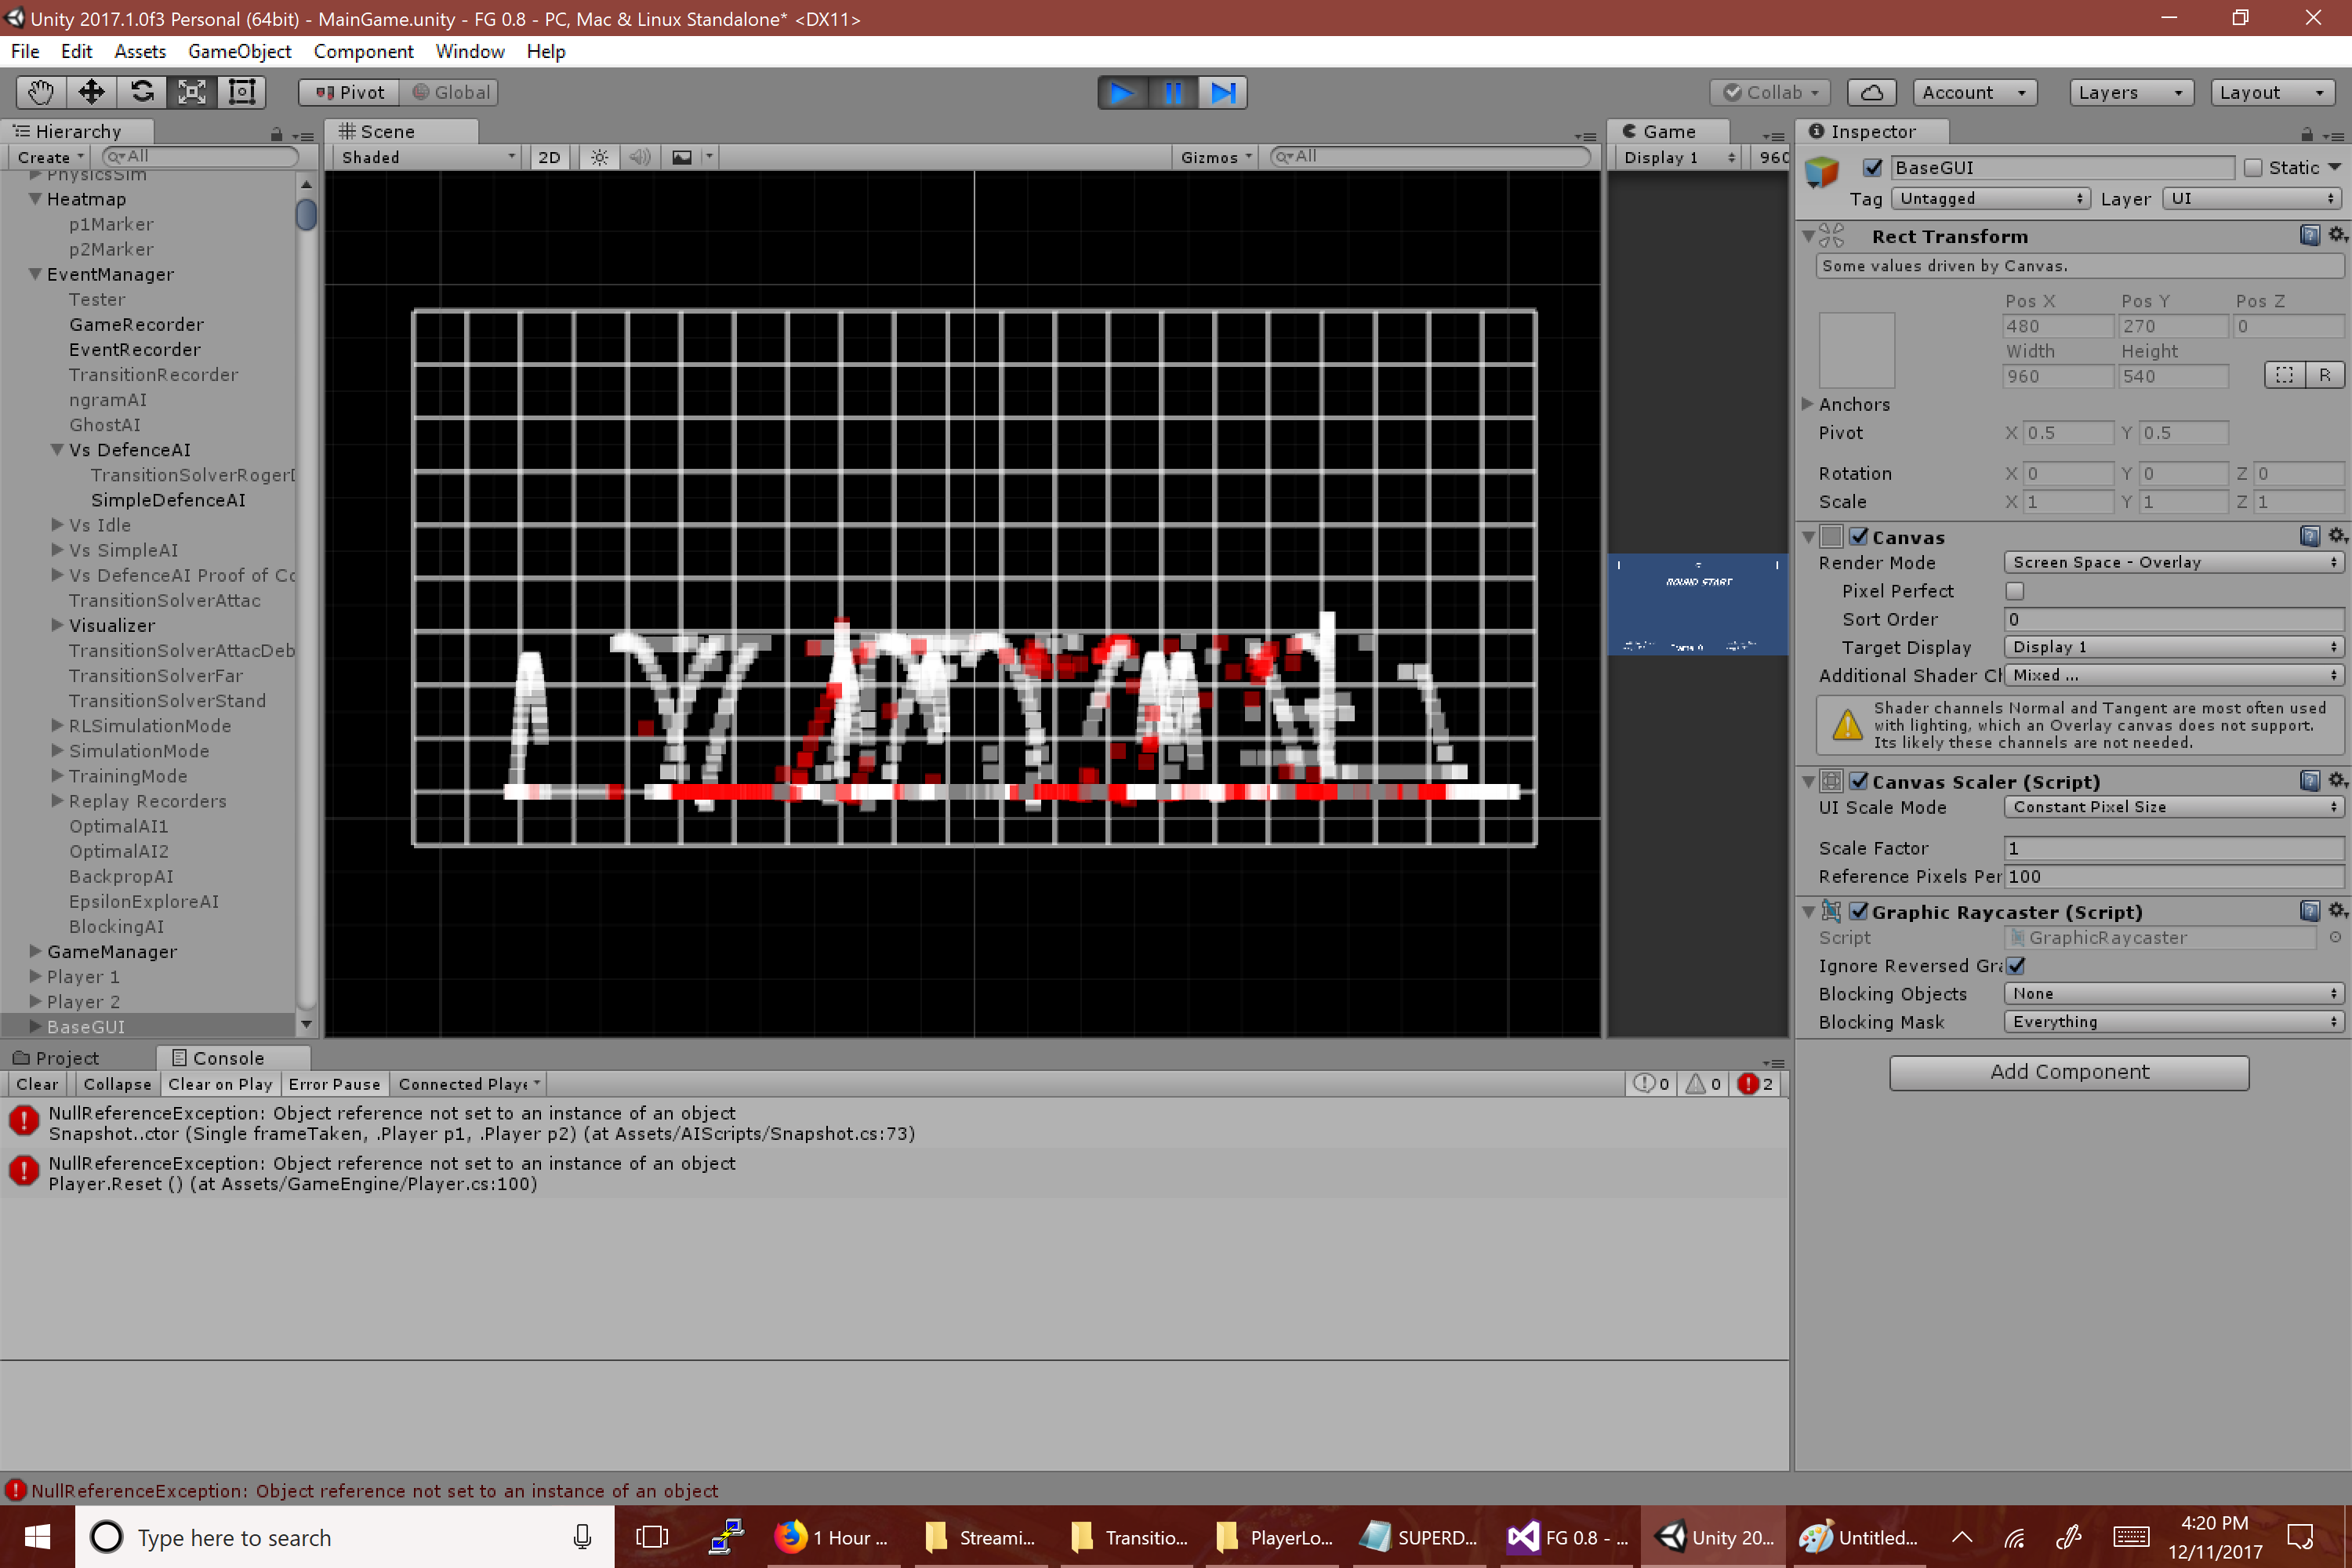
\includegraphics[width=\textwidth]{Figures/HeatmapOrig.png}
		\caption{Original Player Heatmap}
		\label{}
	\end{subfigure}
	\begin{subfigure}[h]{0.4\textwidth}
		\centering
		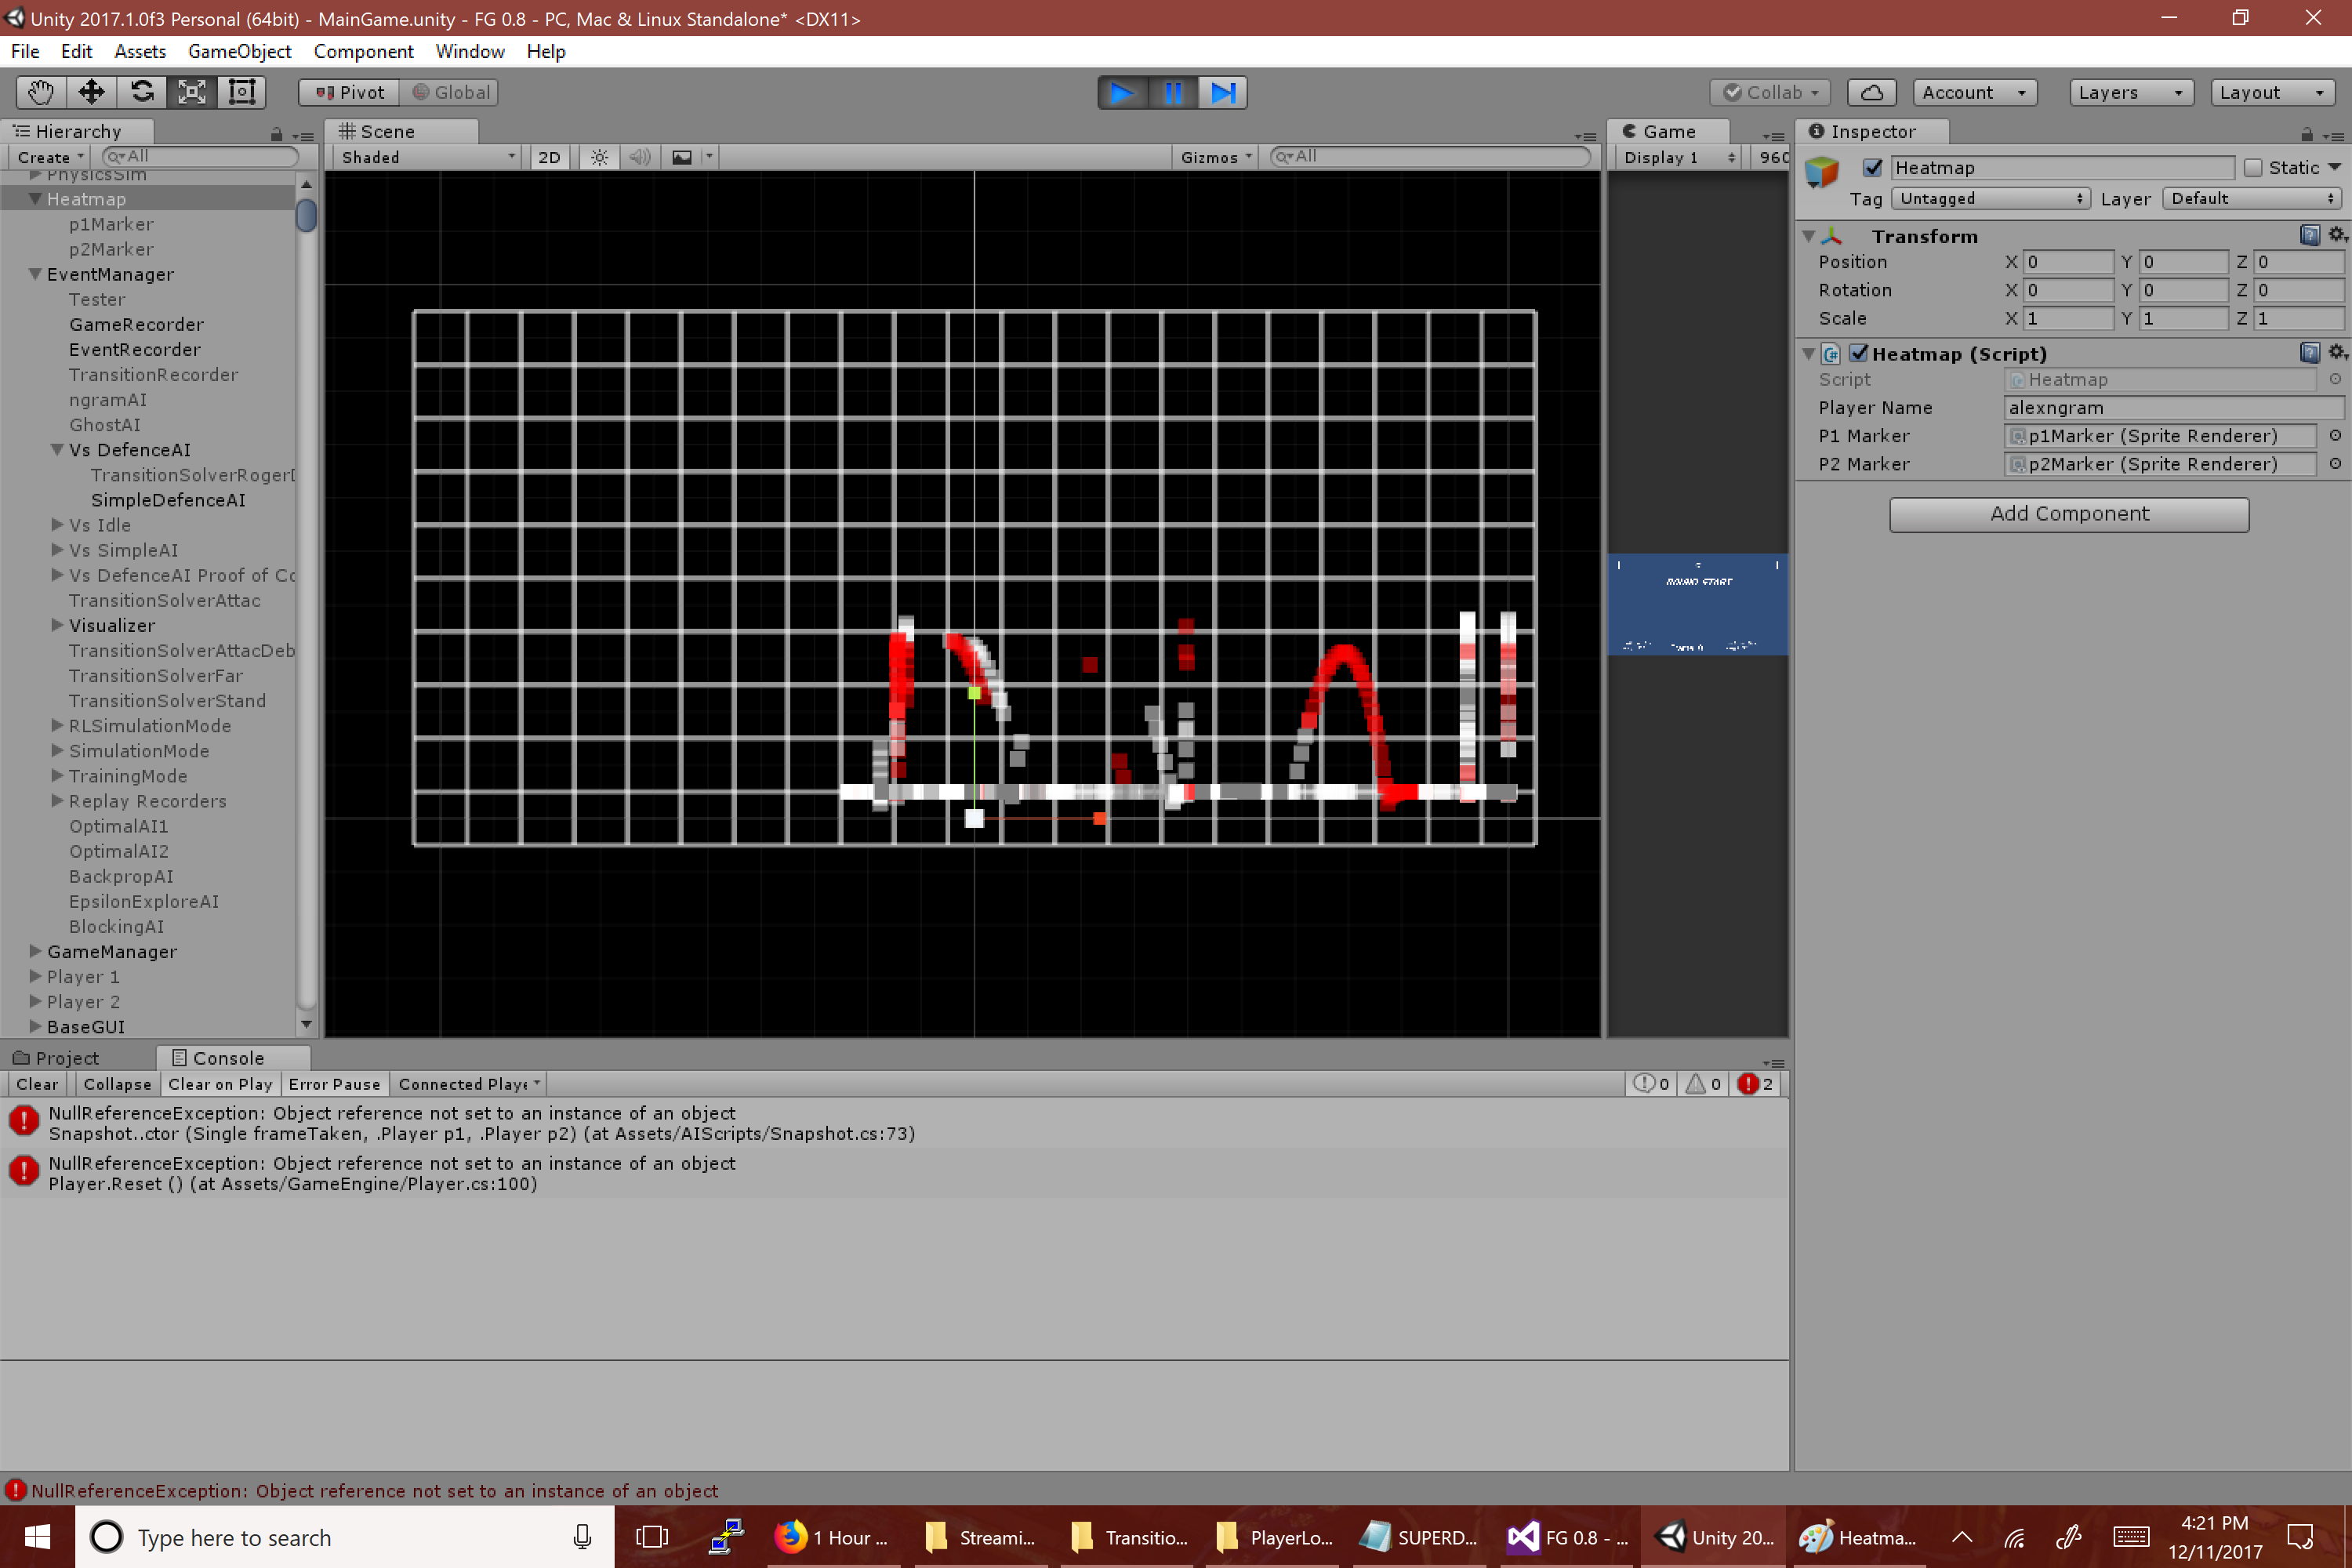
\includegraphics[width=\textwidth]{Figures/HeatmapNgram.png}
		\caption{N-gram AI Heatmap}
		\label{}
	\end{subfigure}
	\begin{subfigure}[h]{0.4\textwidth}
		\centering
		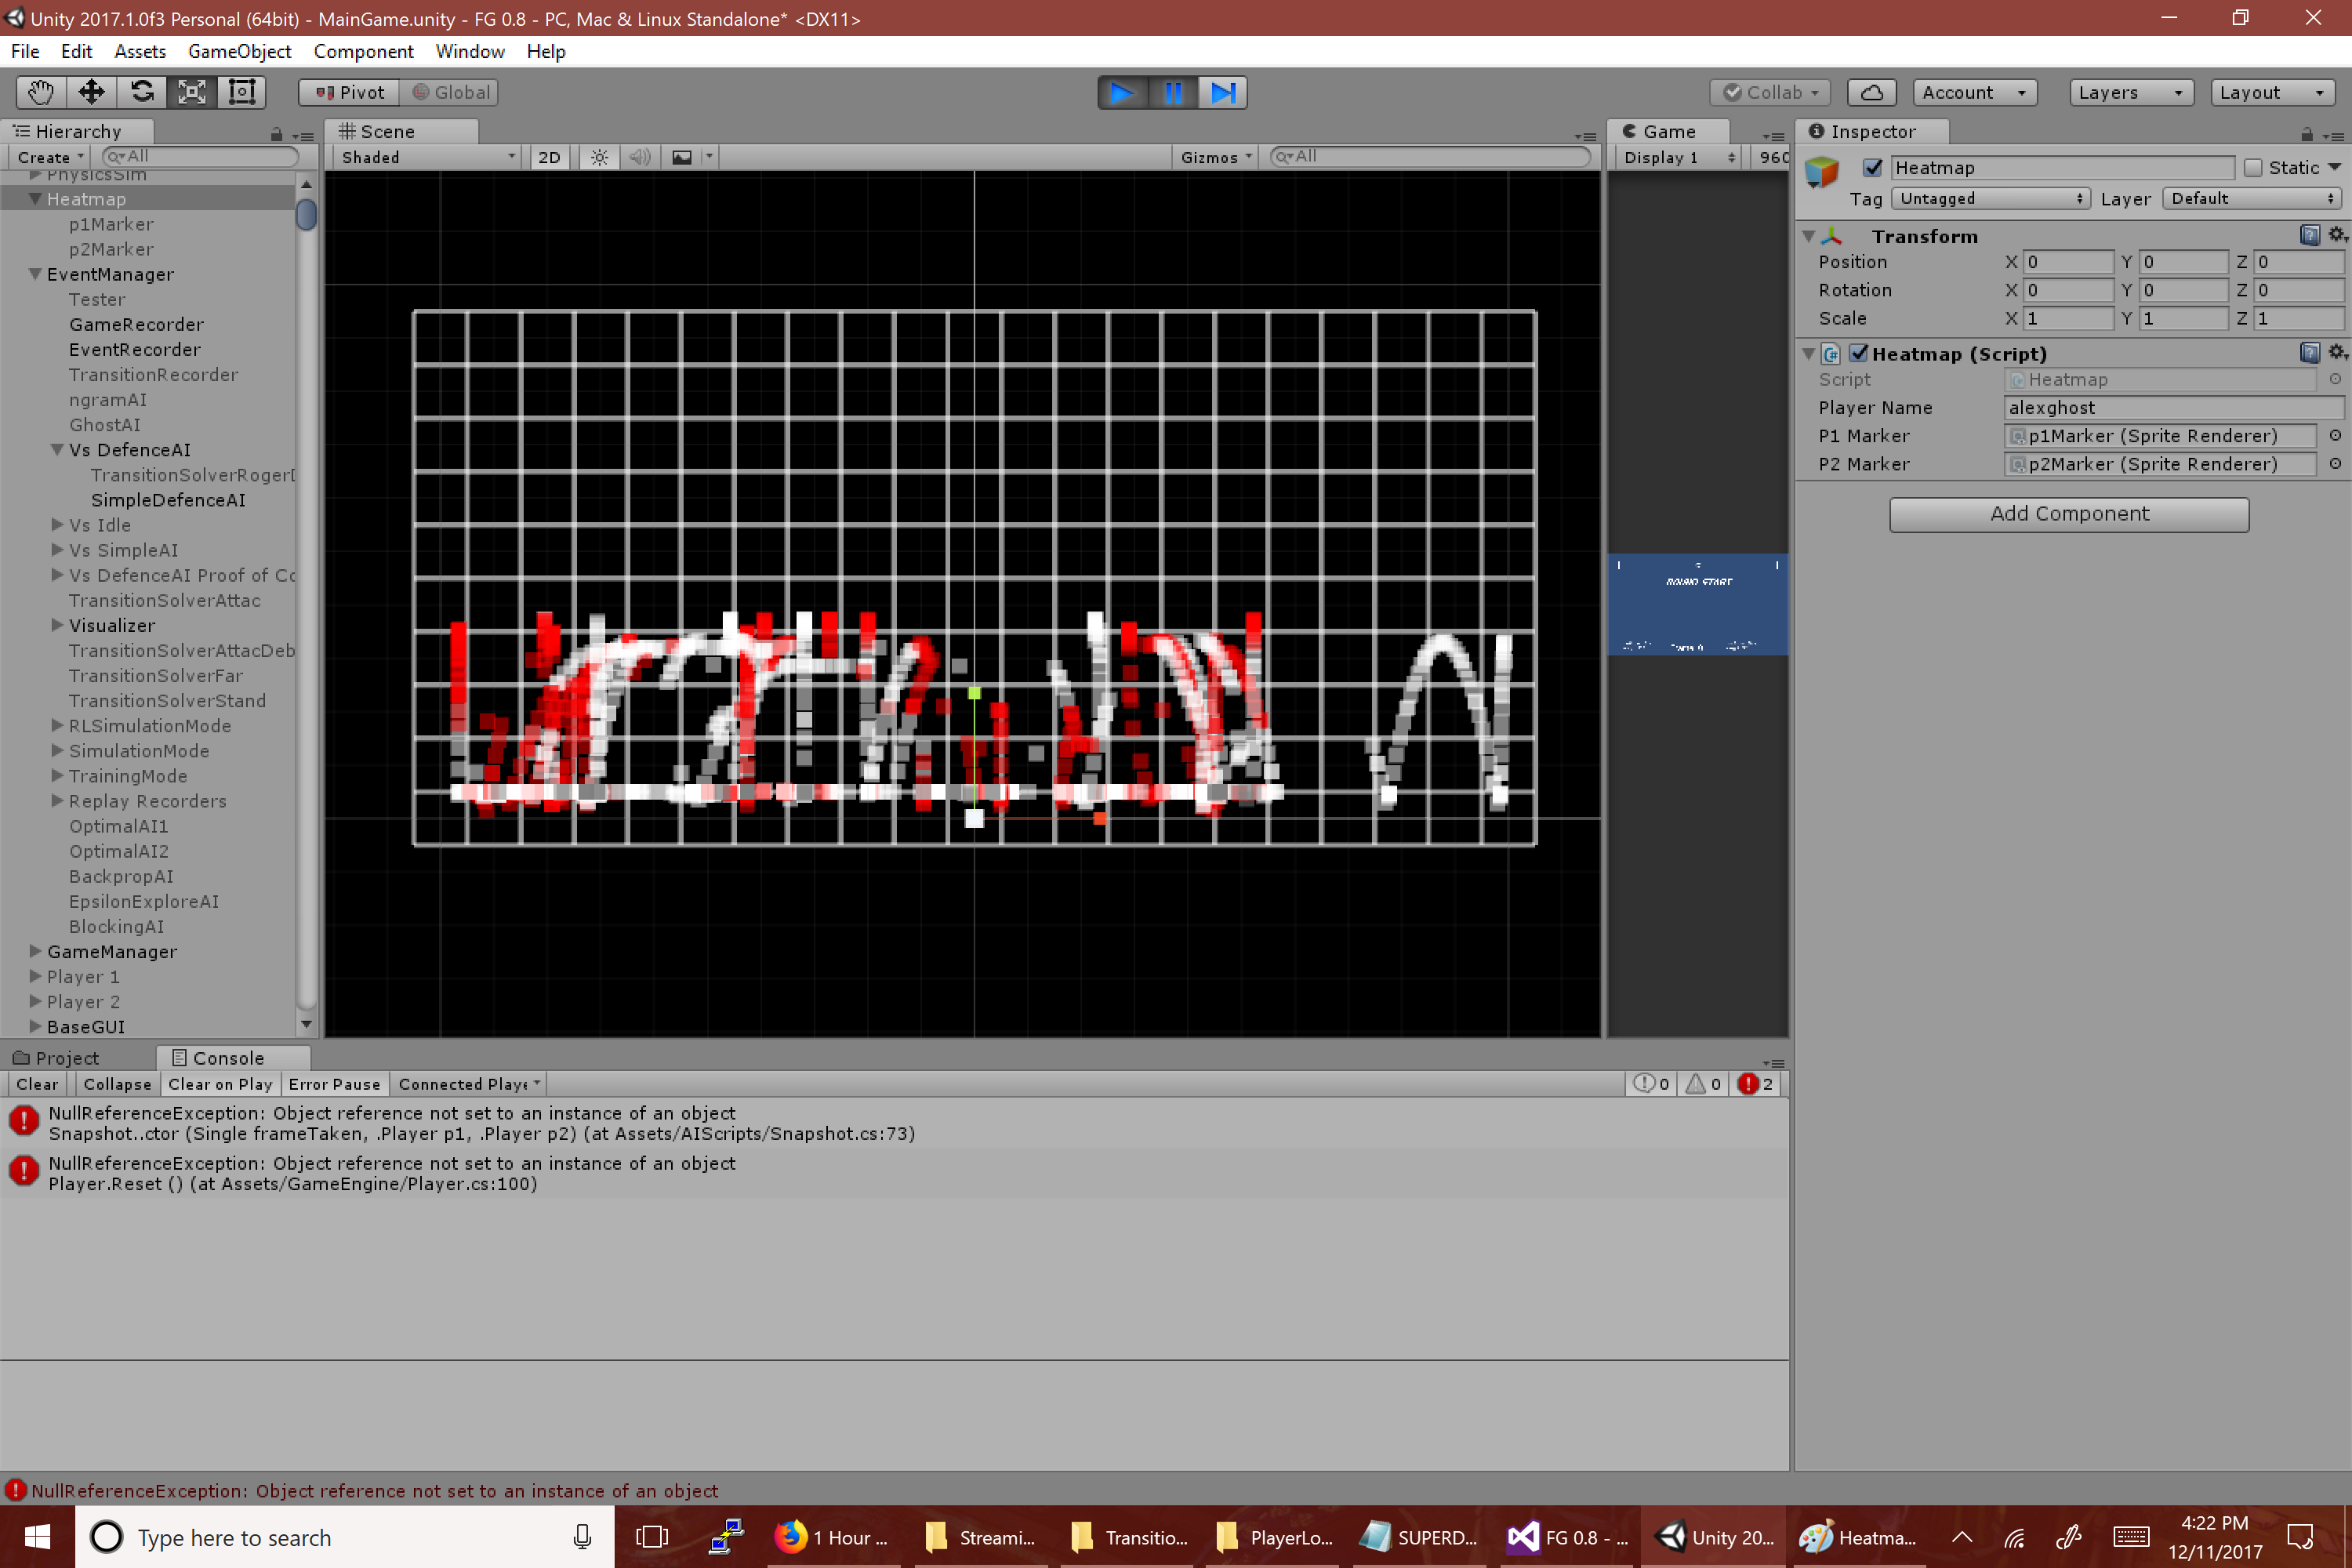
\includegraphics[width=\textwidth]{Figures/HeatmapGhost.png}
		\caption{GhostAI Heatmap}
		\label{}
	\end{subfigure}
	\begin{subfigure}[h]{0.4\textwidth}
		\centering
		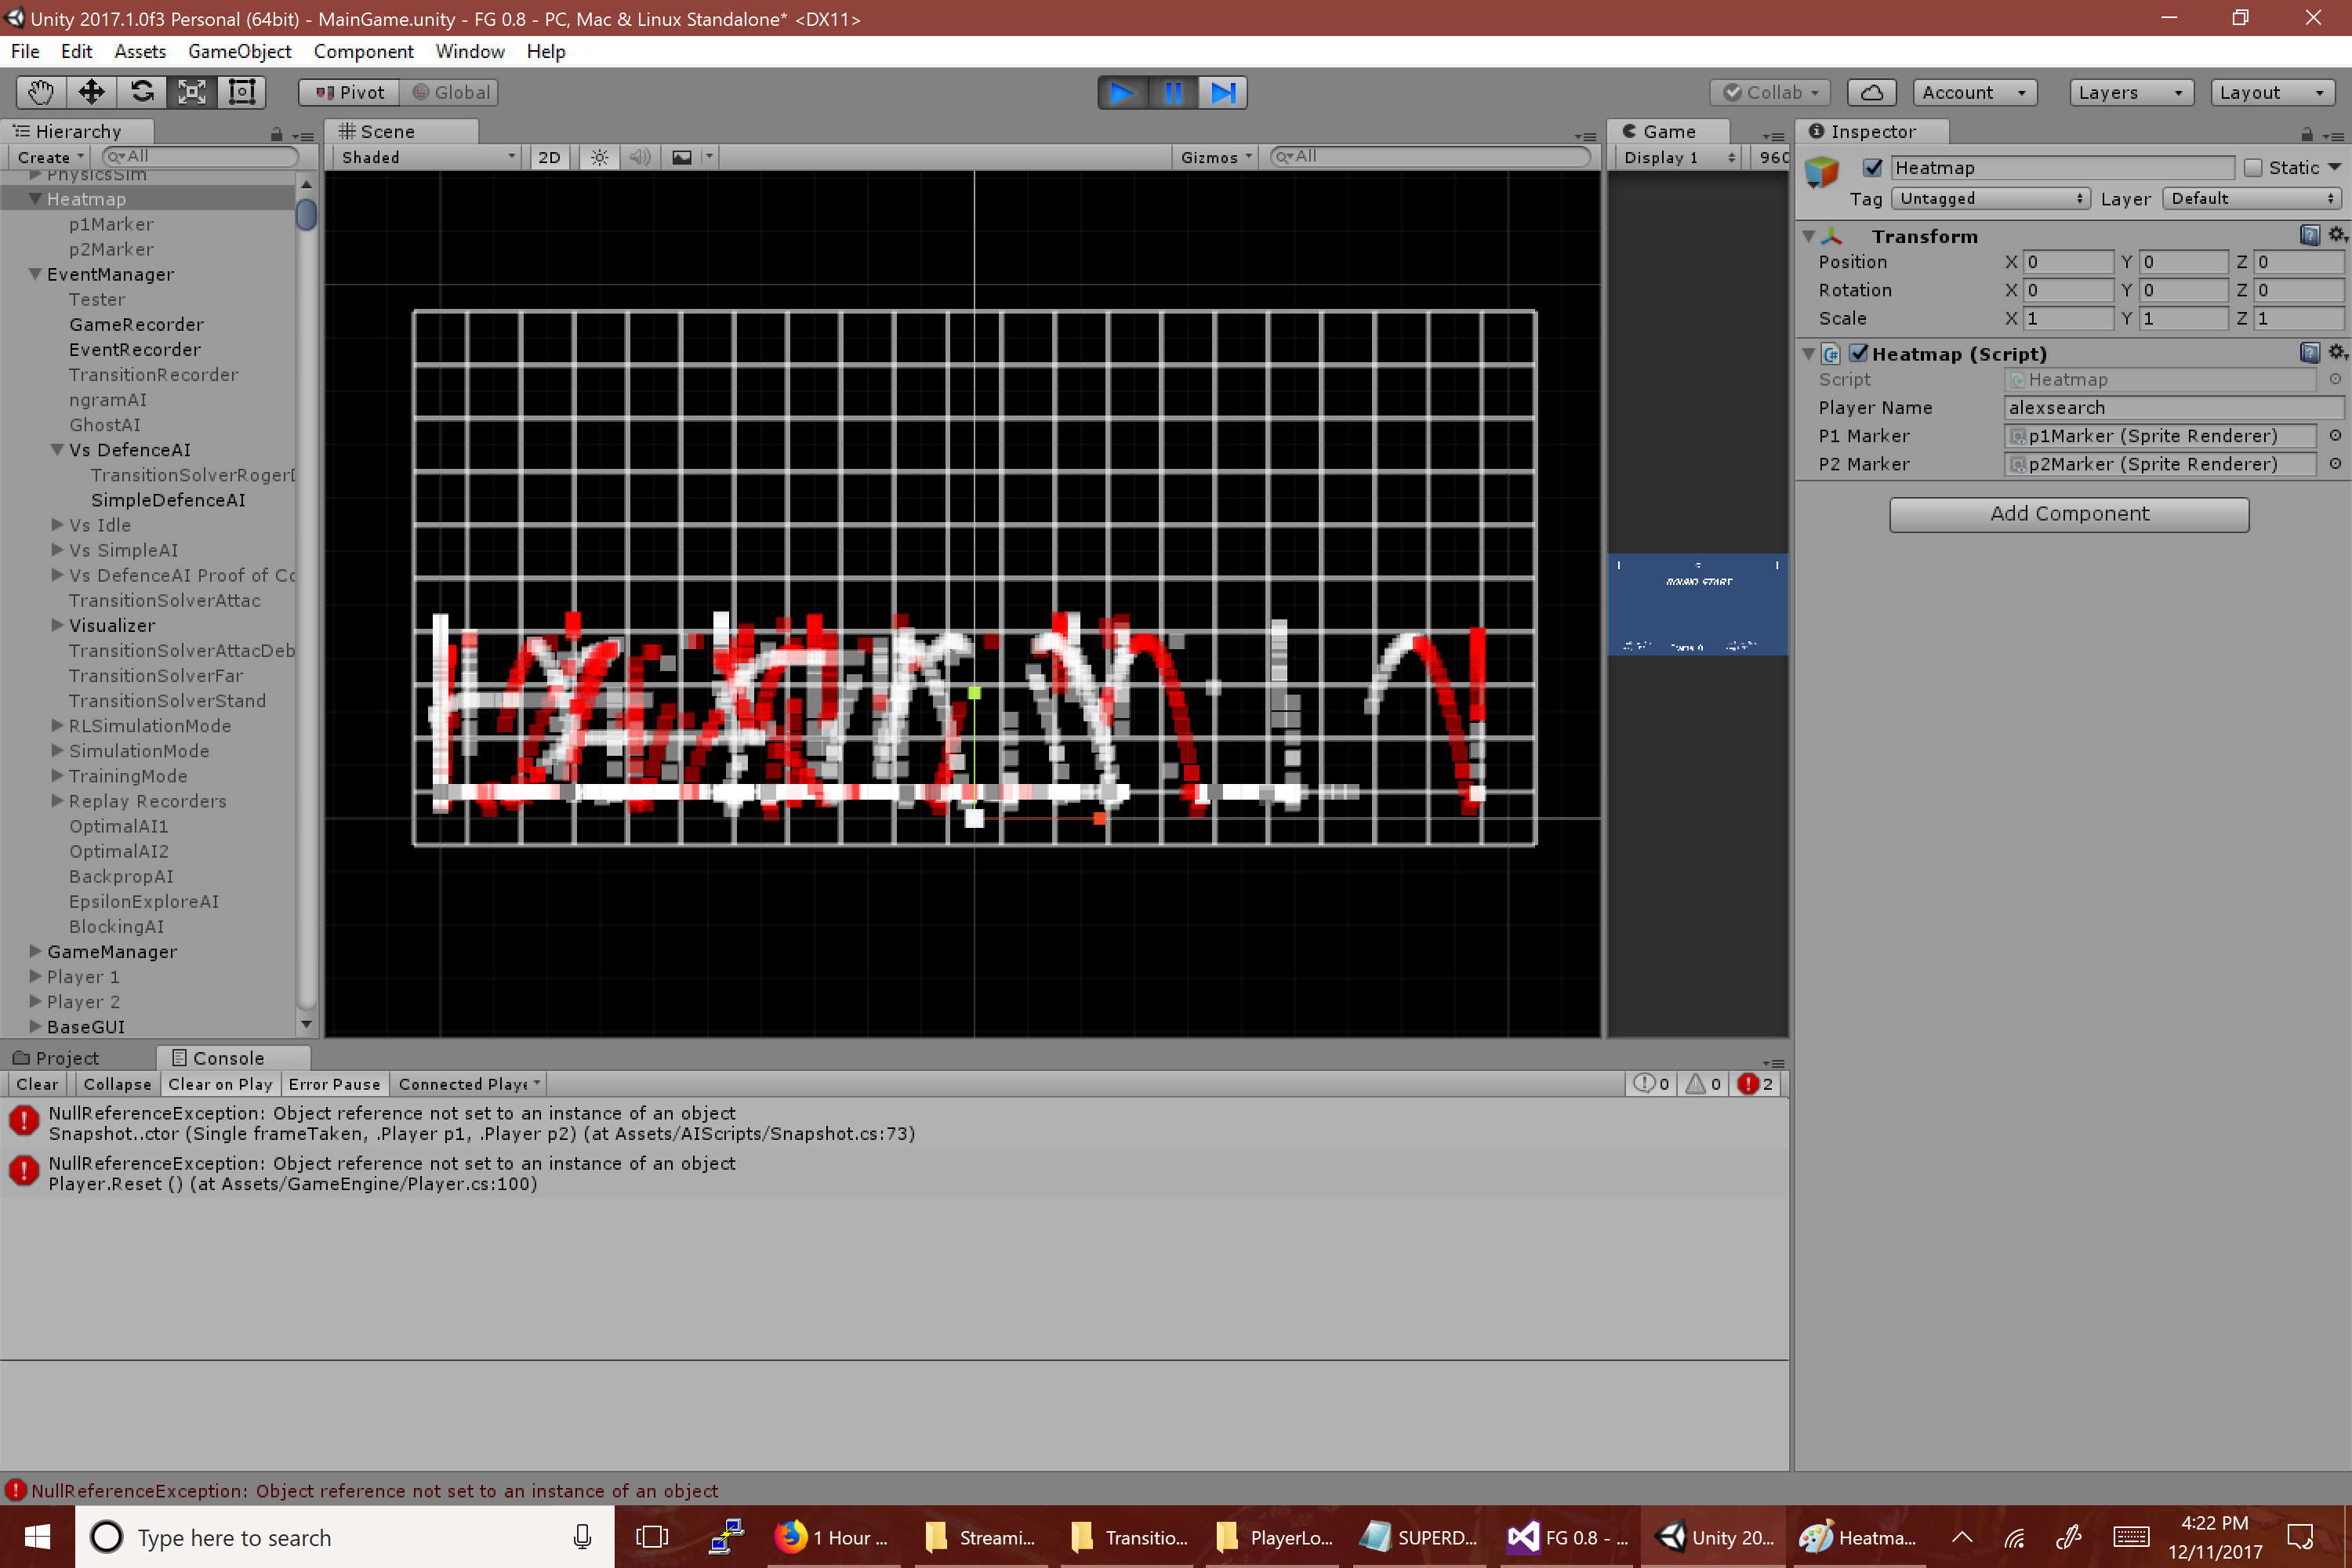
\includegraphics[width=\textwidth]{Figures/HeatmapAI.png}
		\caption{Search AI Heatmap}
		\label{}
	\end{subfigure}
\end{figure}

Lastly from a qualitative standpoint, it is hard to infer much from the heatmaps. They clearly show that Search AI and GhostAI are a step above the N-gram AI, but beyond that there is no clear delineation. Search AI seems to more accurately represent the grounded actions of the original player compared to GhostAI, but it is hard to tell the difference. However, in the video analysis, the Search AI's movement was the smoothest. This is because plannning allows it to take broad motions before deciding to take a different action. That said, both the Ghost AI and Search AI were prone to getting stuck into certain repeated patterns, a trait which to most people signifies a non-human player. This is likely because both GhostAI and Search AI try to reach the goal of hitting the opponent in an efficient manner. This adherence to an "optimal" kind of play can result in situations where the agent behaves greedily to a fault and comes off as non-human-like.


 

%----------------------------------------------------------------------------------------
%	THESIS CONTENT - APPENDICES
%----------------------------------------------------------------------------------------

\appendix % Cue to tell LaTeX that the following "chapters" are Appendices

% Include the appendices of the thesis as separate files from the Appendices folder
% Uncomment the lines as you write the Appendices

% Appendix A

\chapter{Frequently Asked Questions} % Main appendix title

\label{AppendixA} % For referencing this appendix elsewhere, use \ref{AppendixA}

\section{How do I change the colors of links?}

The color of links can be changed to your liking using:

{\small\verb!\hypersetup{urlcolor=red}!}, or

{\small\verb!\hypersetup{citecolor=green}!}, or

{\small\verb!\hypersetup{allcolor=blue}!}.

\noindent If you want to completely hide the links, you can use:

{\small\verb!\hypersetup{allcolors=.}!}, or even better: 

{\small\verb!\hypersetup{hidelinks}!}.

\noindent If you want to have obvious links in the PDF but not the printed text, use:

{\small\verb!\hypersetup{colorlinks=false}!}.

%\include{Appendices/AppendixB}
%\include{Appendices/AppendixC}

%----------------------------------------------------------------------------------------
%	BIBLIOGRAPHY
%----------------------------------------------------------------------------------------

\printbibliography[heading=bibintoc]

%----------------------------------------------------------------------------------------

\end{document}  
